\chapter{Lijst van bestanden beschikbaar op online locaties}

\begin{enumerate}
	\item \onlineitem{Theorie gegeneerd uit diagram \ref{fig:seq-diagram-game} volgens de regels in secties \ref{sec:sd-voc} en \ref{sec:cons-to-ltc}}{https://pastebin.com/WGQjr2bv}
	\item \onlineitem{Theorie gegenereerd uit het ontwerp voor Nim in sectie \ref{sec:nim-design}}{https://pastebin.com/f90riJGV}
	\item \onlineitem{Diagrammen voor het ontwerp voor Reversi in sectie \ref{sec:reversi-design}}{https://imgur.com/a/kgVg4dv}
	\item \onlineitem{Theorie gegeneerd uit het ontwerp voor Reversi in sectie \ref{sec:reversi-design}}{https://pastebin.com/B1zKWyTq}
\end{enumerate}

\chapter{IDP-bestand resulterend uit de procedure beschreven in sectie \ref{sec:cd-rep-cons} voor diagram \ref{fig:diagram-voorbeeld}}\label{app:consistentie}

\lstinputlisting[caption=Theorie voor het diagram in figuur \ref{fig:diagram-voorbeeld}]{chap-rol-idp/generatedtheory.idp}\label{code:consistentie}

\chapter{IDP-bestand resulterend uit de procedure beschreven in sectie \ref{sec:kwaliteitsgebrek} voor diagrammen \ref{fig:diagram-voorbeeld} en \ref{fig:cycle}}\label{app:kwaliteitsgebrek}

\lstinputlisting[caption=Theorie voor het opsporen van kwaliteitsgebreken]{chap-rol-idp/defs.idp}\label{code:kwaliteitsgebrek}

%\chapter{IDP-bestand voor sequentiediagram van het spelvoorbeeld}\label{app:seq-diagram-game}
%
%\lstinputlisting[caption=Modellering van het gedrag van het sequentiediagram in figuur \ref{fig:seq-diagram-game}]{idp-sources/seq-diagram-game.idp}\label{code:seq-diagram-game}

\chapter{IDP-bestand voor diagrammen \ref{fig:recursion-class}, \ref{fig:methodOne} en \ref{fig:methodtwo} in sectie \ref{sec:interaction}}\label{app:seq-recursion}

\lstinputlisting[caption=Modellering van het gedrag van de sequentiediagrammen in figuren \ref{fig:methodOne} en \ref{fig:methodtwo}]{idp-sources/recursion.idp}\label{code:seq-recursion}

\chapter{Diagrammen voor het ontwerp van Nim in sectie \ref{sec:nim-design}}\label{app:design-nim}

%\afterpage{
%	\begin{landscape}
%		\newpage
%		\thispagestyle{empty}
%		\begin{figure}
%			%\vspace*{-0.5cm}
%			\begin{subfigure}{\textwidth}
%				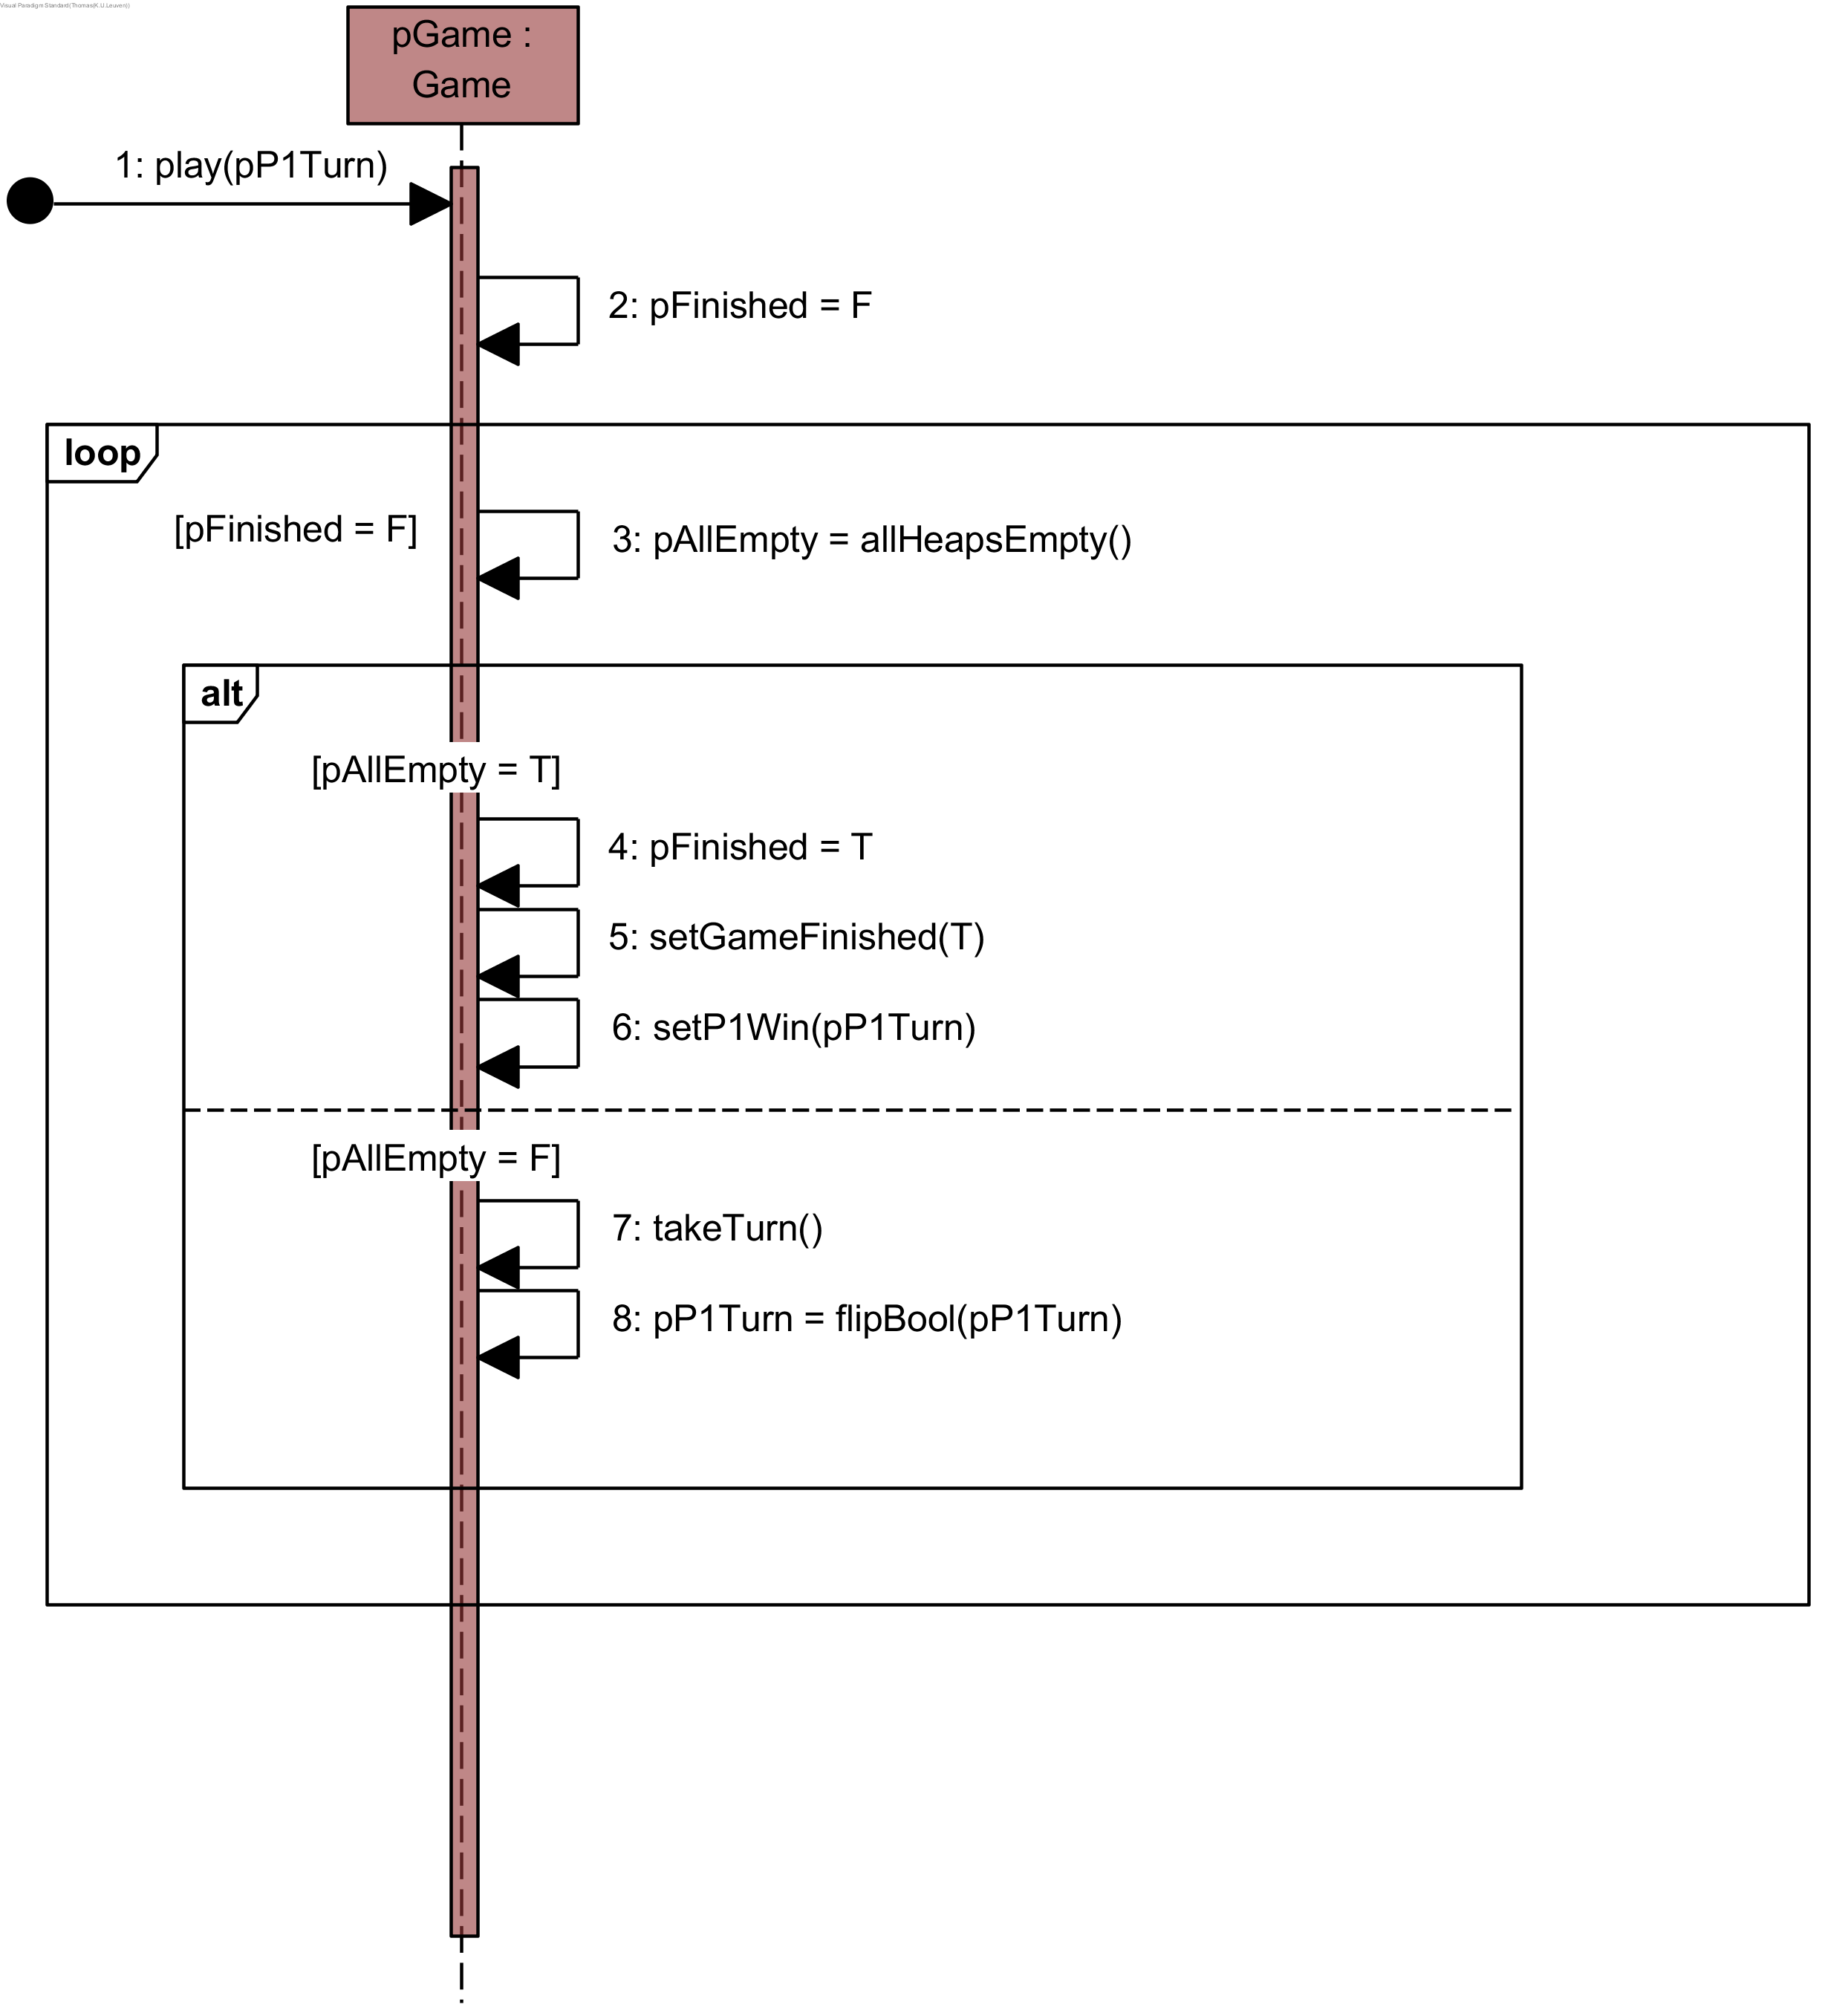
\includegraphics[width=0.8\textwidth]{chap-evaluatie/play.png}
%				\caption{Sequentiediagram voor \textit{play(boolean)}}
%				\label{fig:nim-play}
%			\end{subfigure}%
%			\begin{subfigure}{\textwidth}
%				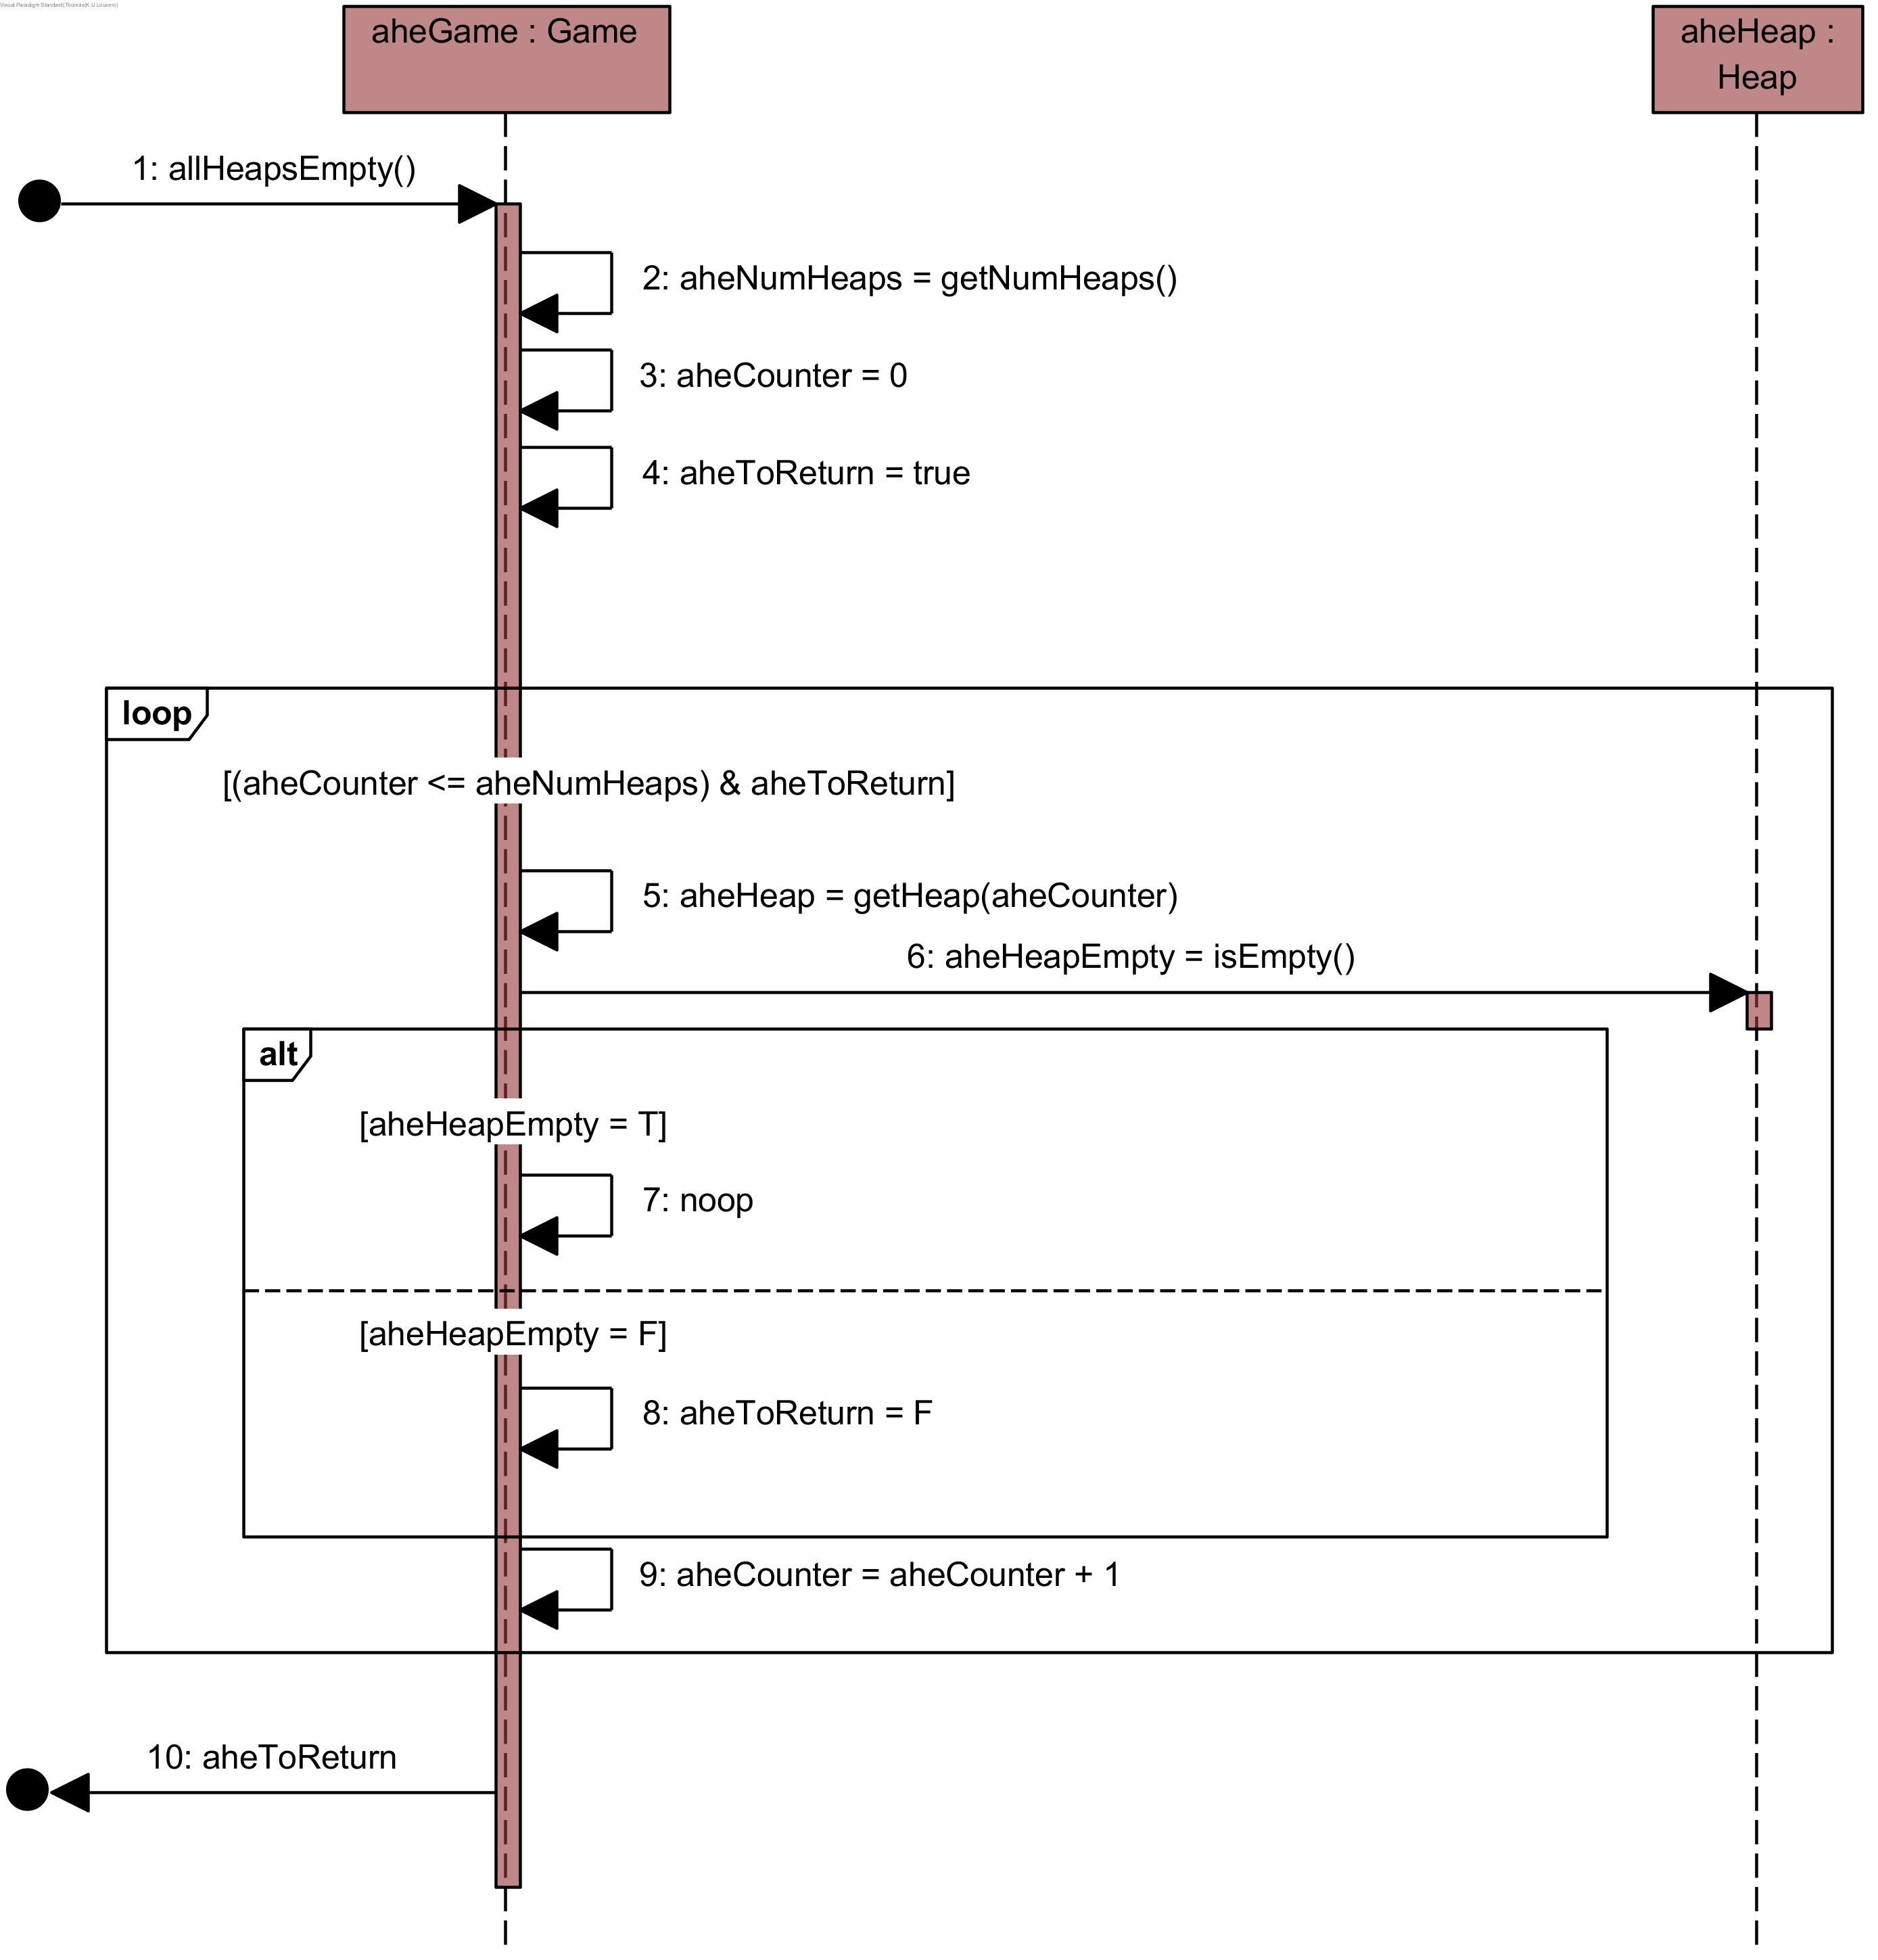
\includegraphics[width=0.8\textwidth]{chap-evaluatie/allHeapsEmpty.png}
%				\caption{Sequentiediagram voor \textit{allHeapsEmpty()}}
%				\label{fig:nim-allHeapsEmpty}
%			\end{subfigure}
%			\caption{Sequentiediagrammen voor \textit{play(boolean)} en \textit{allHeapsEmpty()}}
%			\label{fig:nim-play-ahe}
%		\end{figure}
%	\end{landscape}
%}

\begin{figure}
	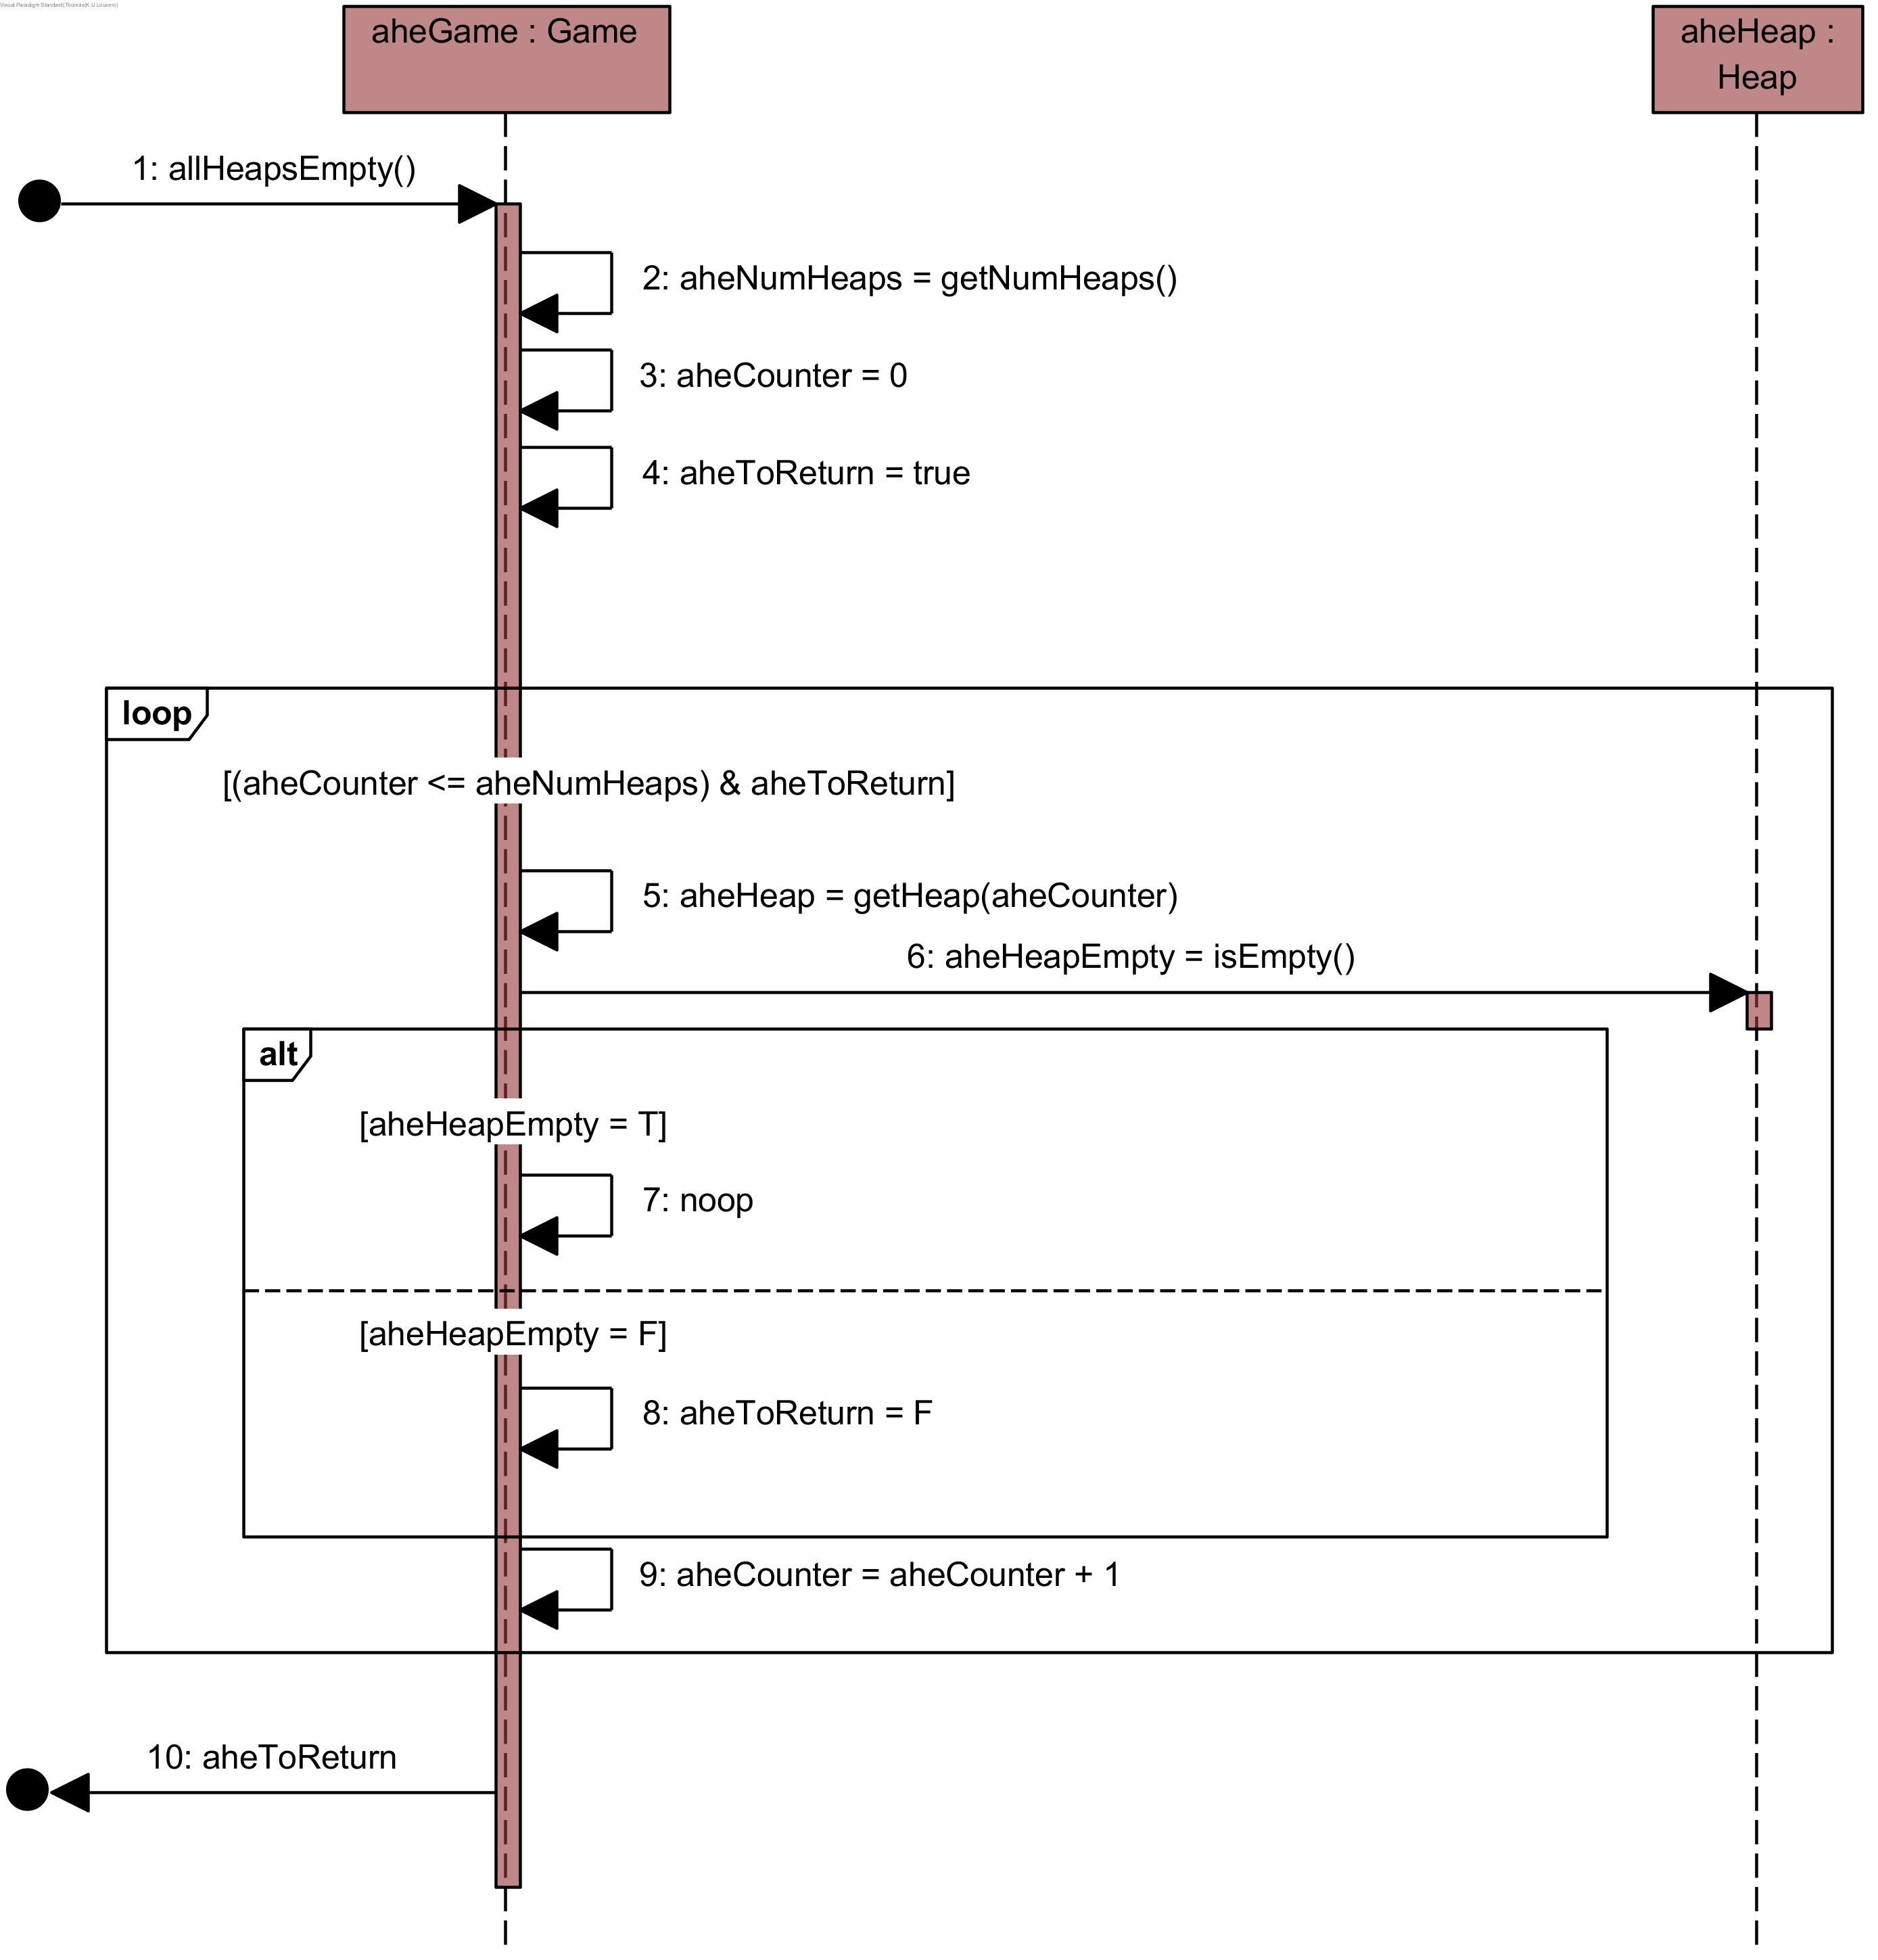
\includegraphics[width=0.8\textwidth]{chap-evaluatie/allHeapsEmpty.png}
	\caption{Sequentiediagram voor \textit{allHeapsEmpty()}}
	\label{fig:nim-allHeapsEmpty}
\end{figure}

%\afterpage{
%	\clearpage
	\begin{landscape}
		\newpage
		\thispagestyle{empty}
		
		\begin{figure}
			\begin{subfigure}{\textwidth}
				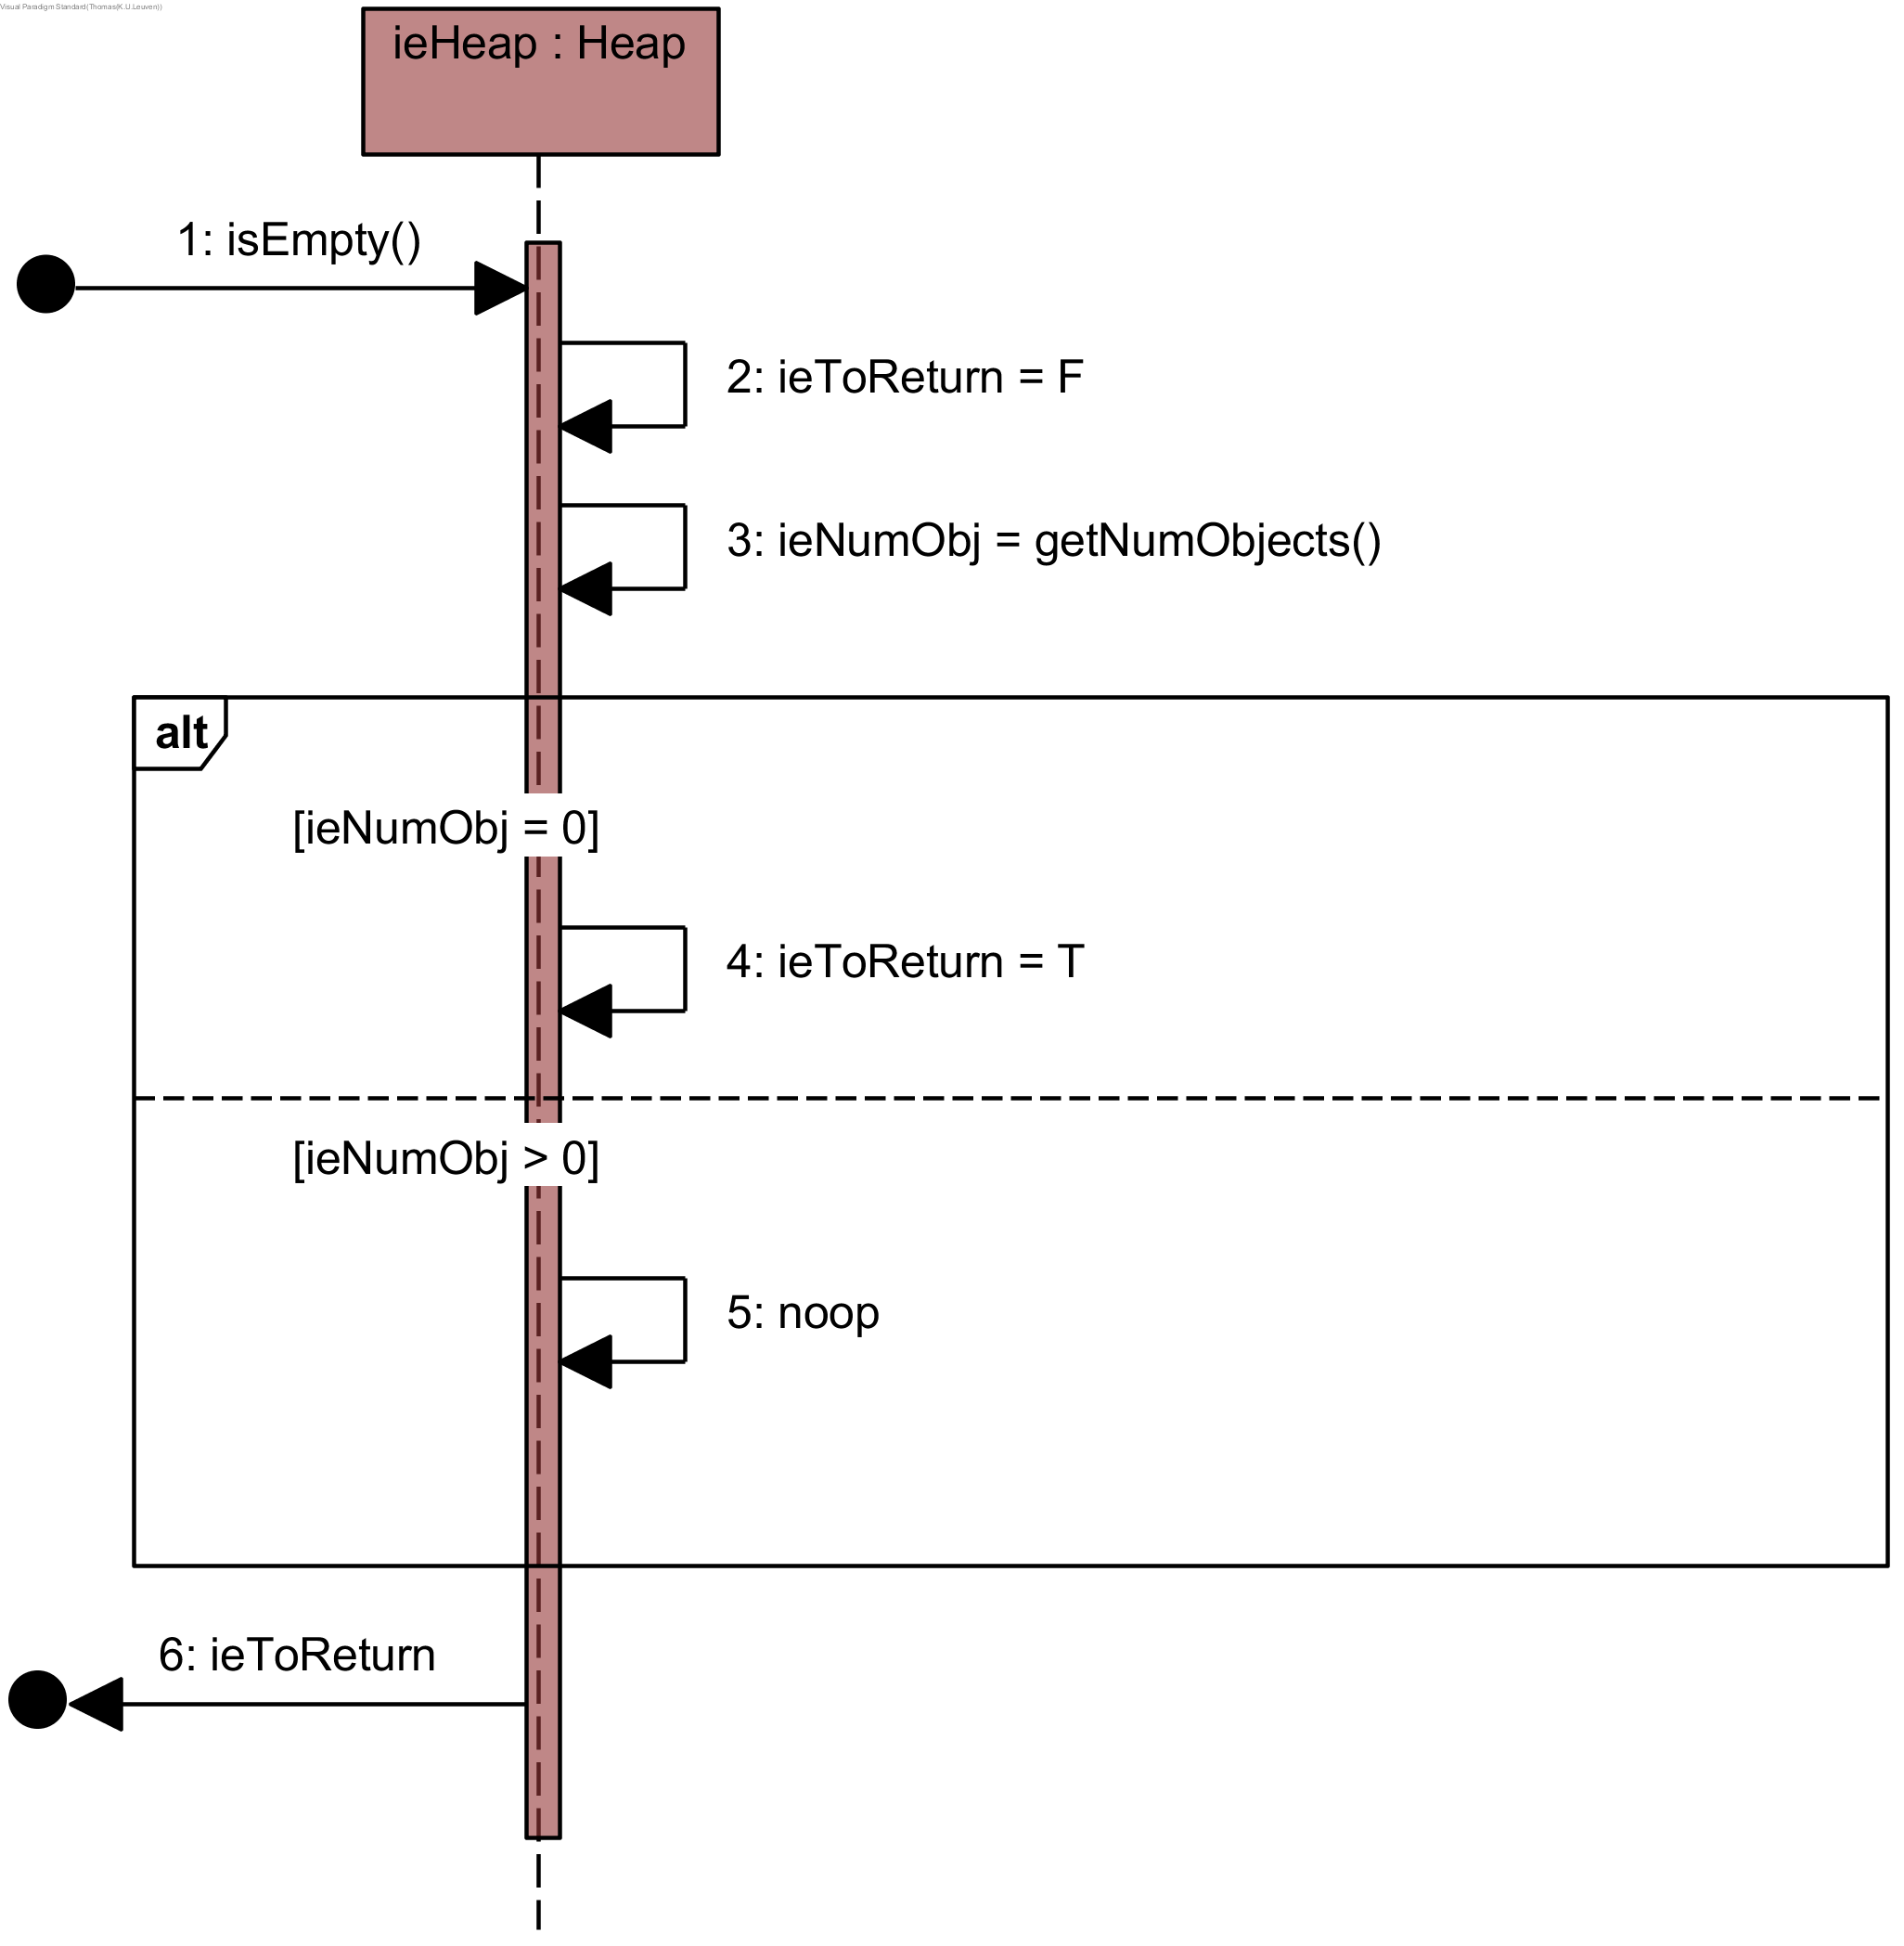
\includegraphics[width=0.75\textwidth]{chap-evaluatie/isEmpty.png}
				\caption{Sequentiediagram voor \textit{isEmpty()}}
				\label{fig:nim-isEmpty}
			\end{subfigure}%
			\begin{subfigure}{\textwidth}
				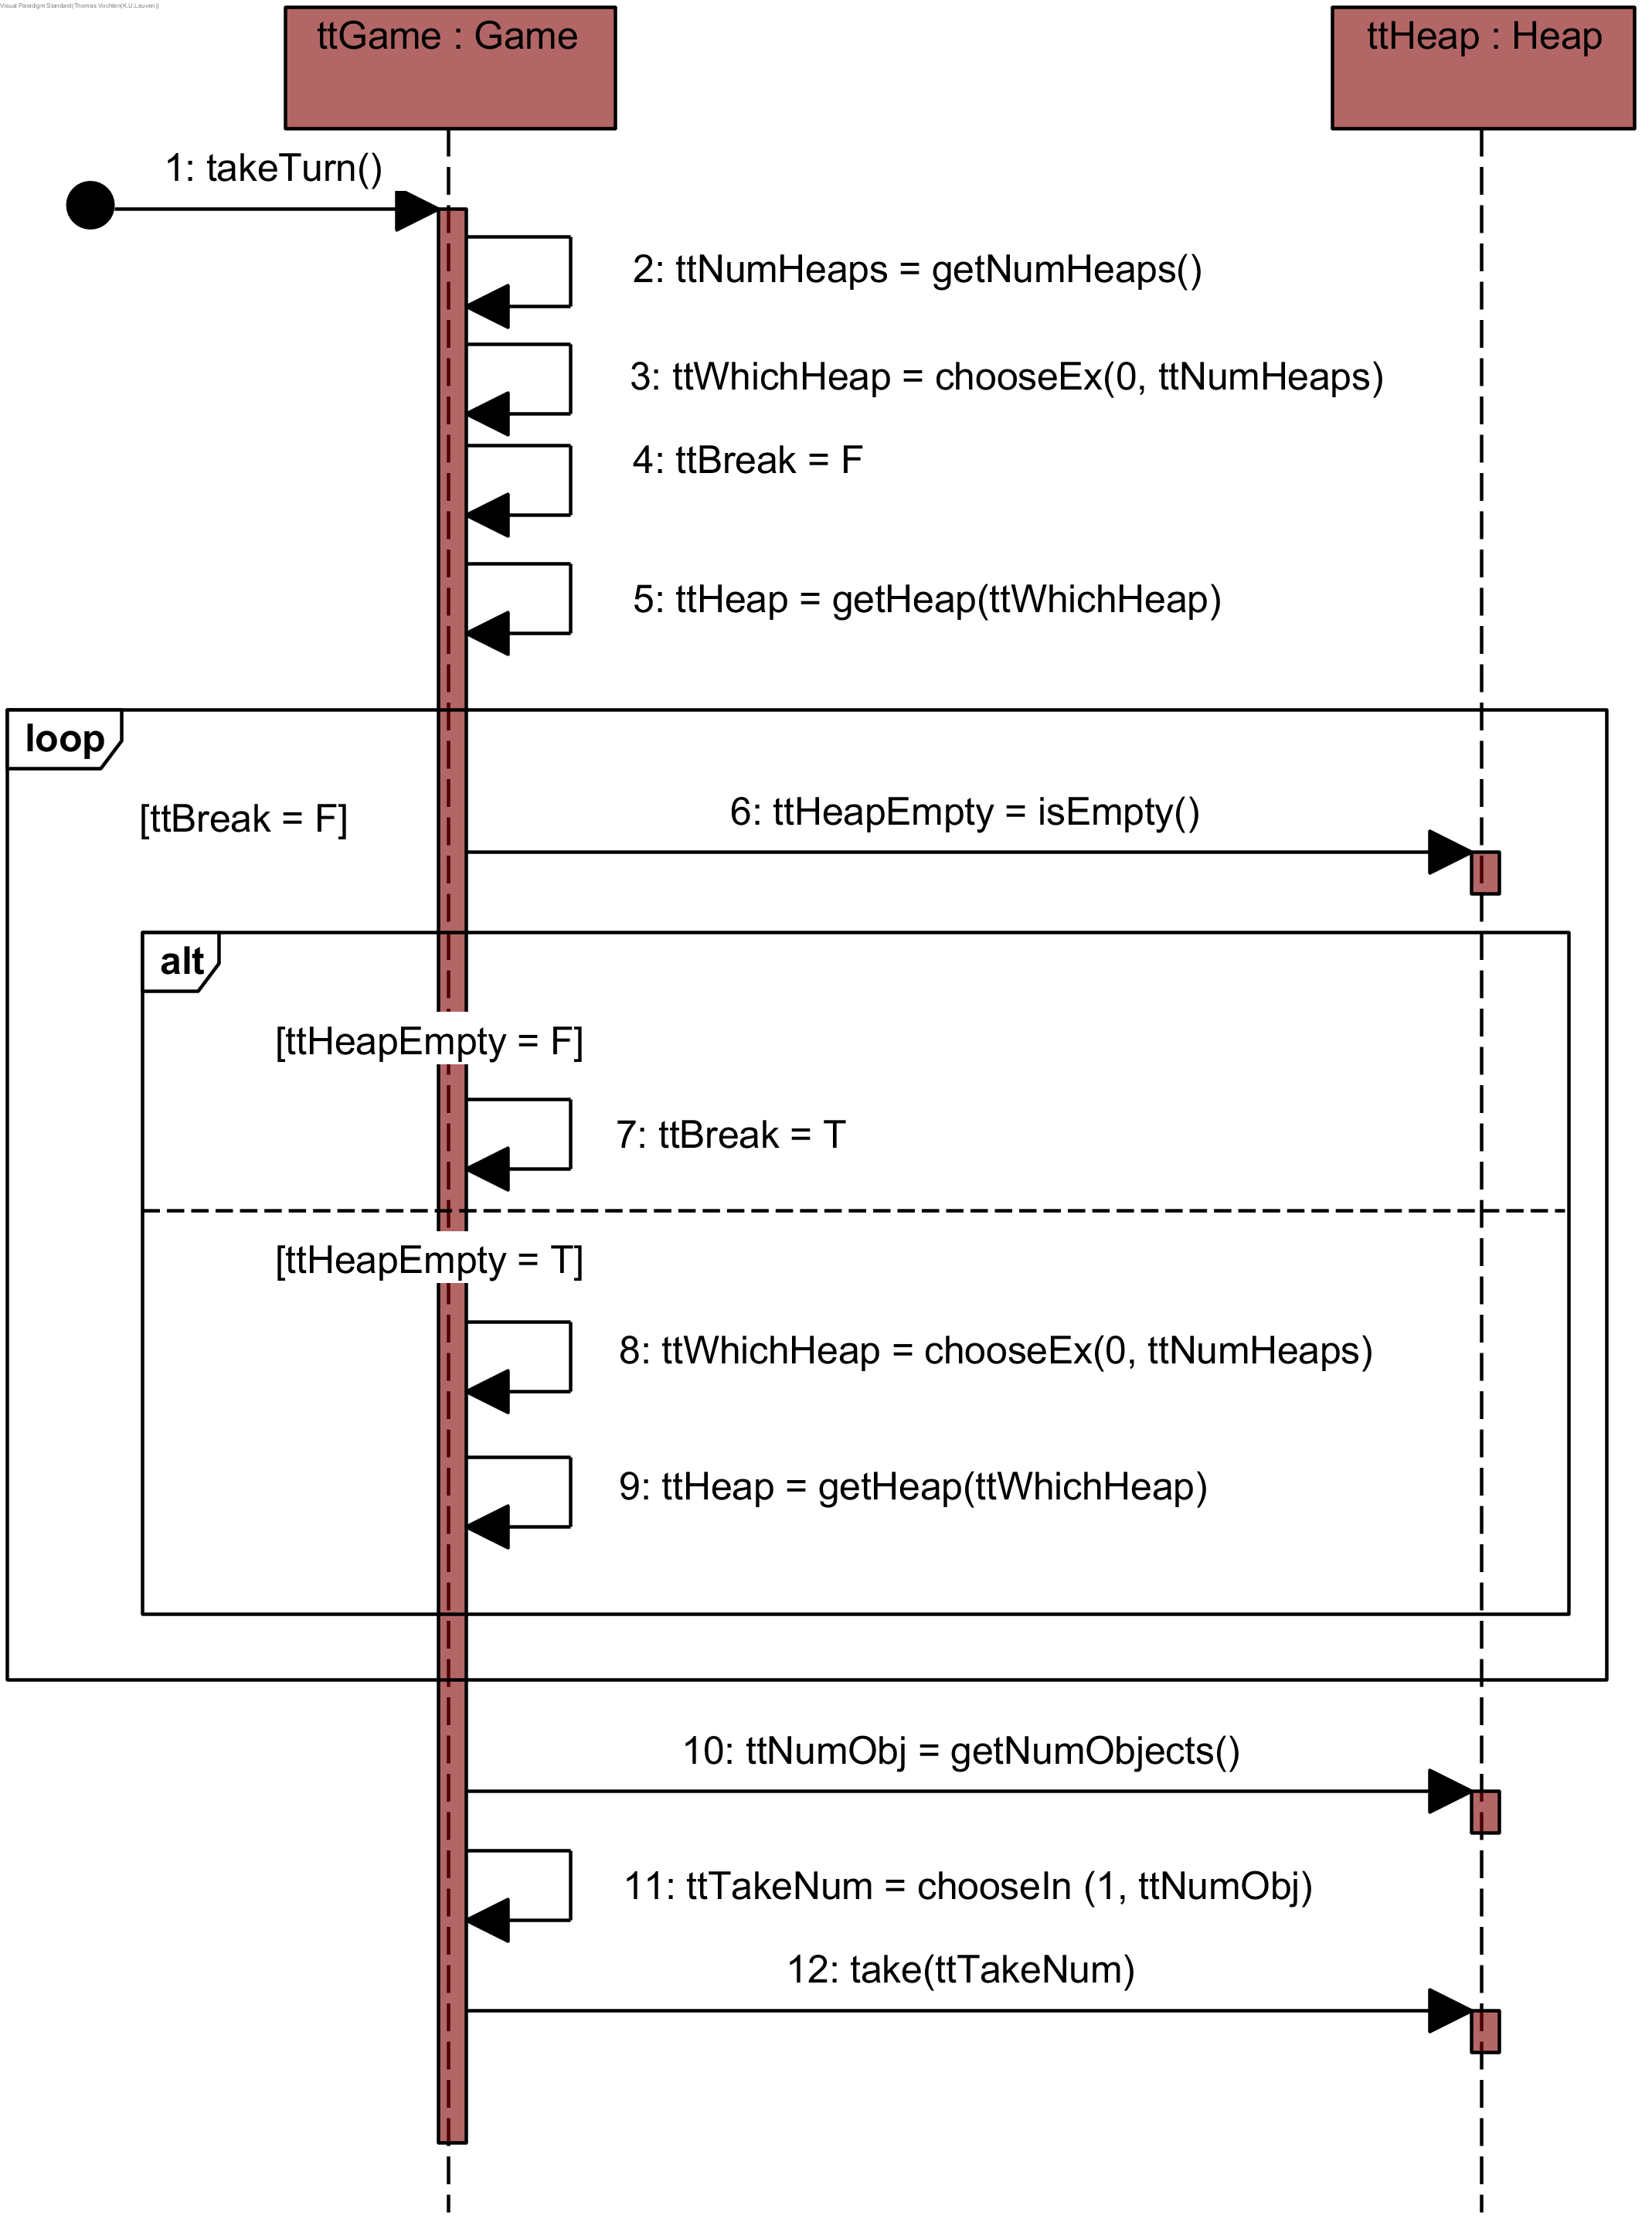
\includegraphics[width=0.8\textwidth]{chap-evaluatie/takeTurn.png}
				\caption{Sequentiediagram voor \textit{takeTurn()}}
				\label{fig:nim-takeTurn}
			\end{subfigure}
			\caption{Sequentiediagrammen voor \textit{isEmpty()} en \textit{takeTurn()}}
			\label{fig:nim-isempty-tt}
		\end{figure}
	\end{landscape}
%}

\begin{figure}[htp]
	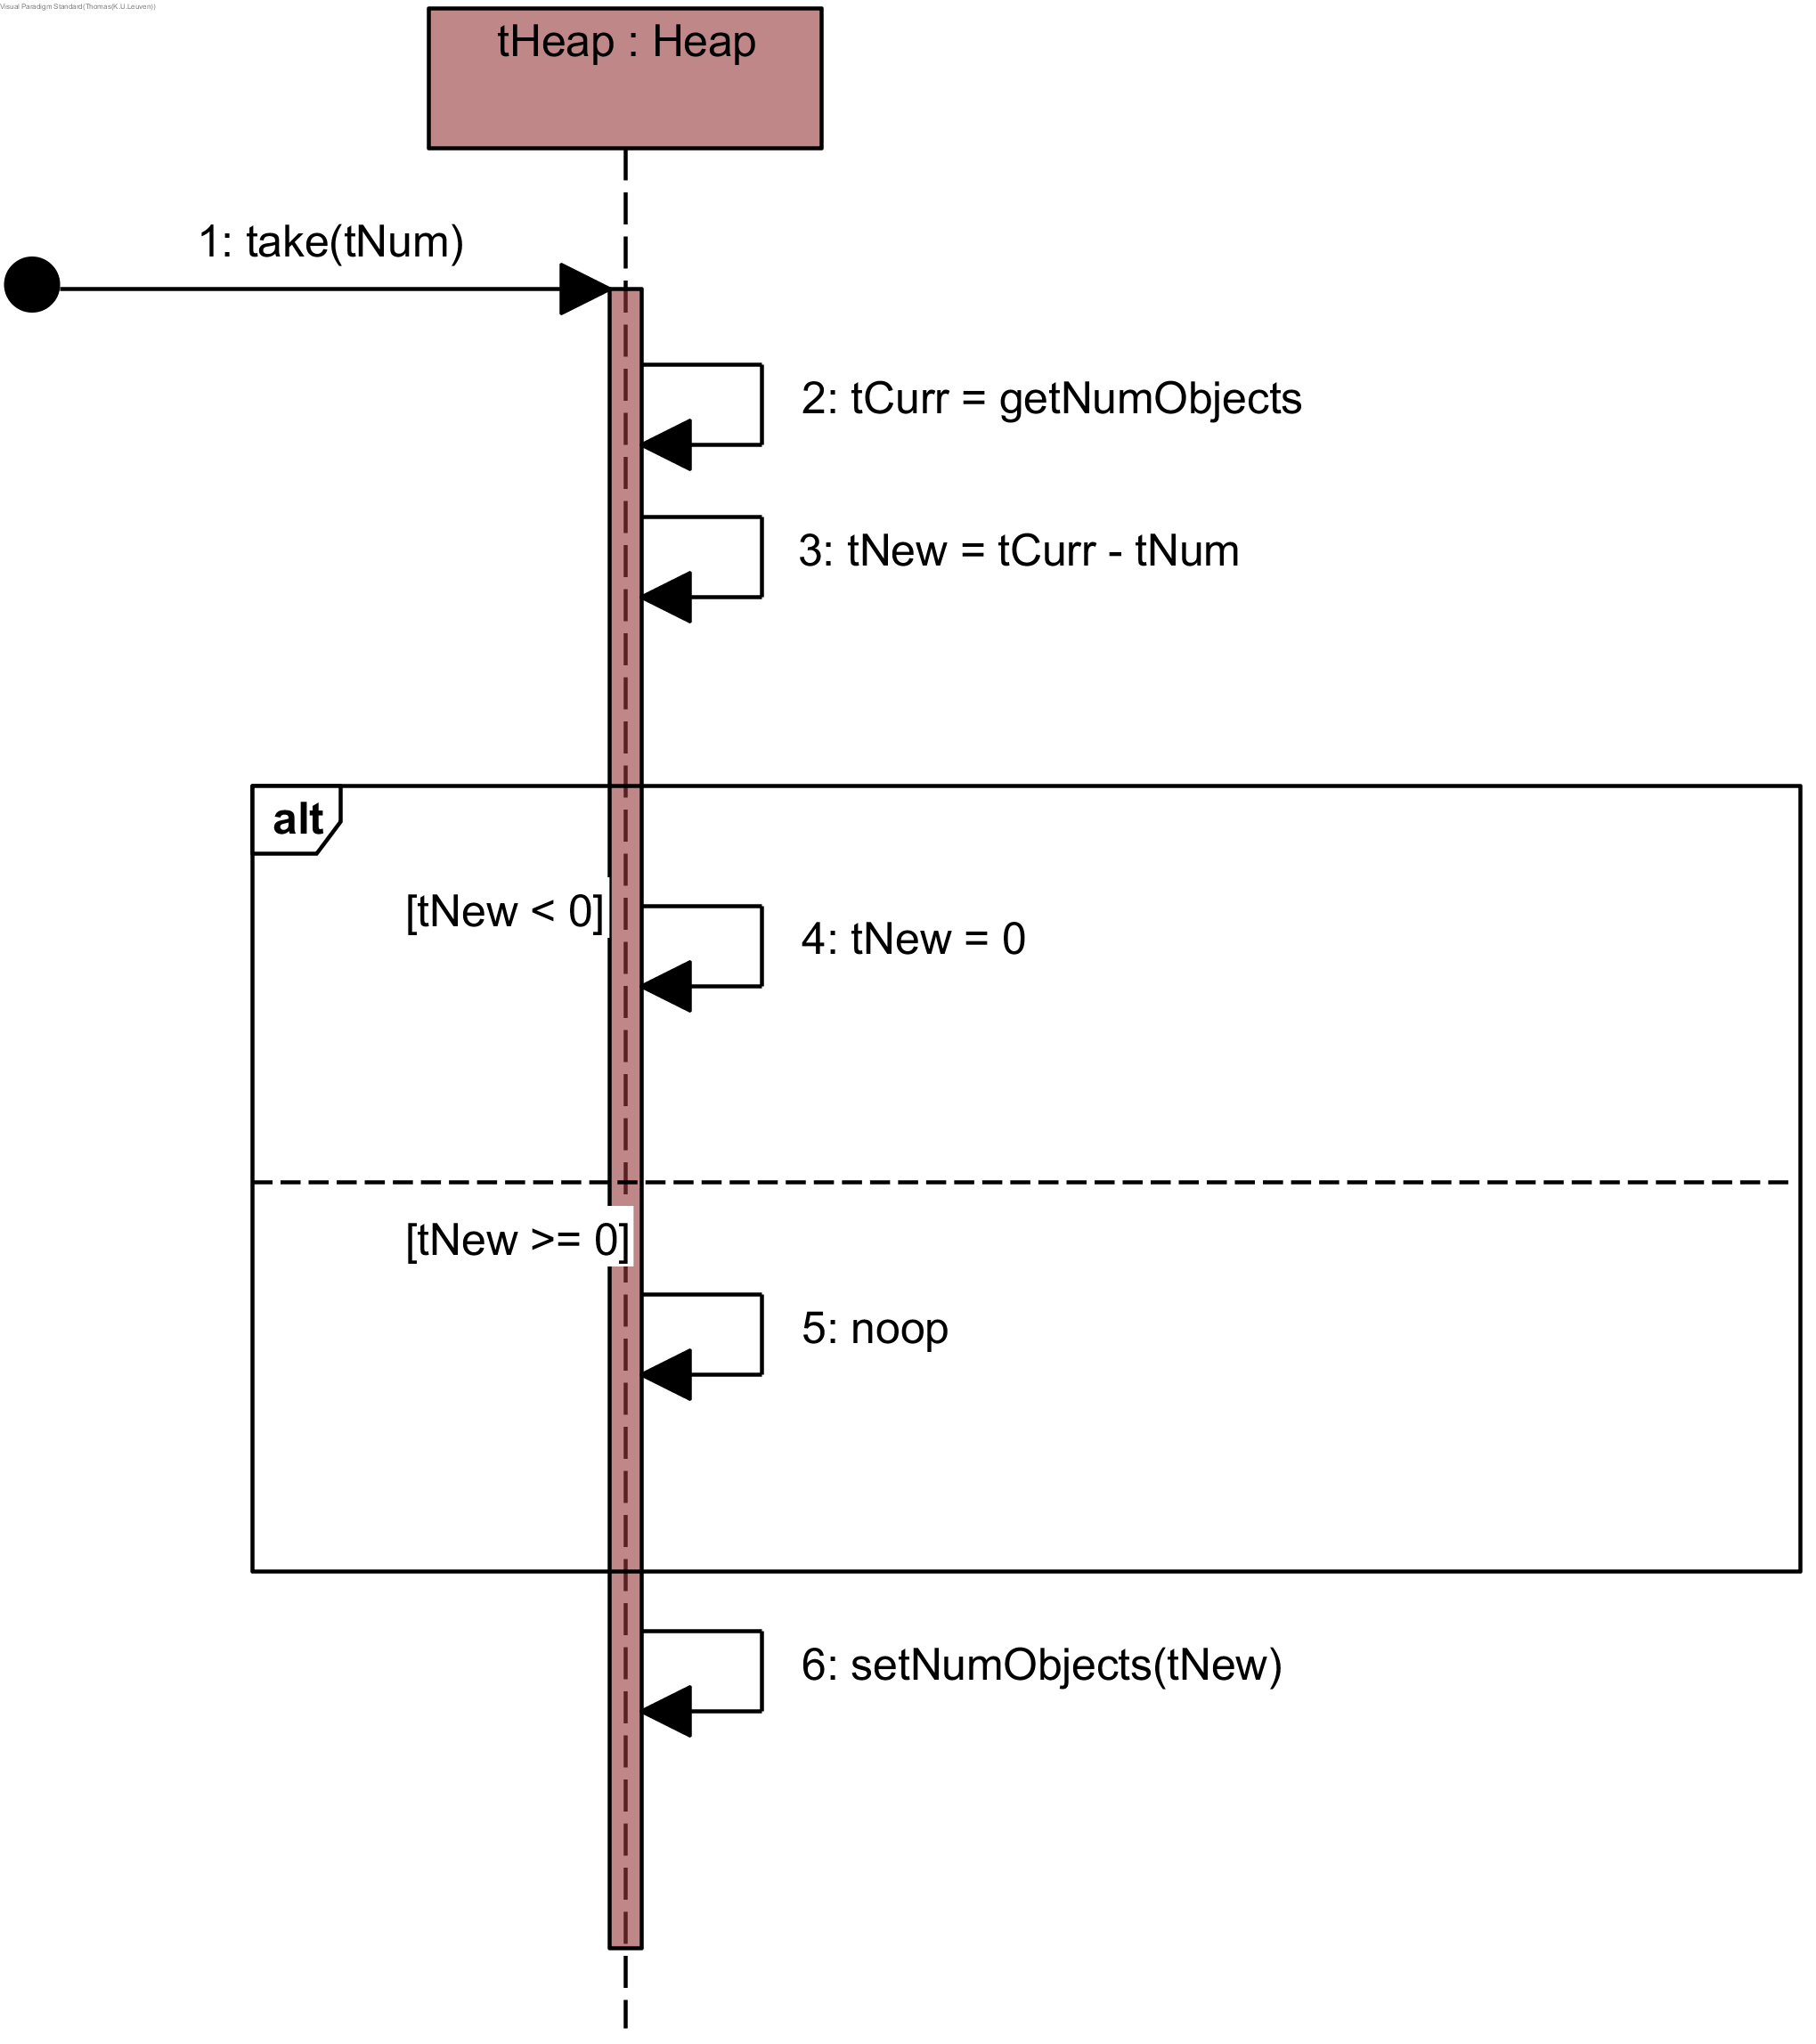
\includegraphics[width=0.8\textwidth]{chap-evaluatie/take.png}
	\caption{Sequentiediagram voor \textit{take(int)}}
	\label{fig:nim-take}
\end{figure}

%\chapter{IDP-bestand voor het ontwerp van Nim}\label{app:nim-eval}
%
%\lstinputlisting[caption=Modellering van Nim voor hoofdstuk \ref{sec:evaluatie}]{chap-evaluatie/nimmodel.idp}\label{code:nim-eval}

%\chapter{IDP-bestand voor het ontwerp van Reversi}\label{app:reversi-eval}
%
%\lstinputlisting[caption=Modellering van Reversi voor hoofdstuk \ref{sec:evaluatie}]{chap-evaluatie/reversimodel.idp}\label{code:reversi-eval}

%\chapter{Diagrammen voor het ontwerp van Reversi}
%
%\begin{figure}[htp]
%	\centering
%	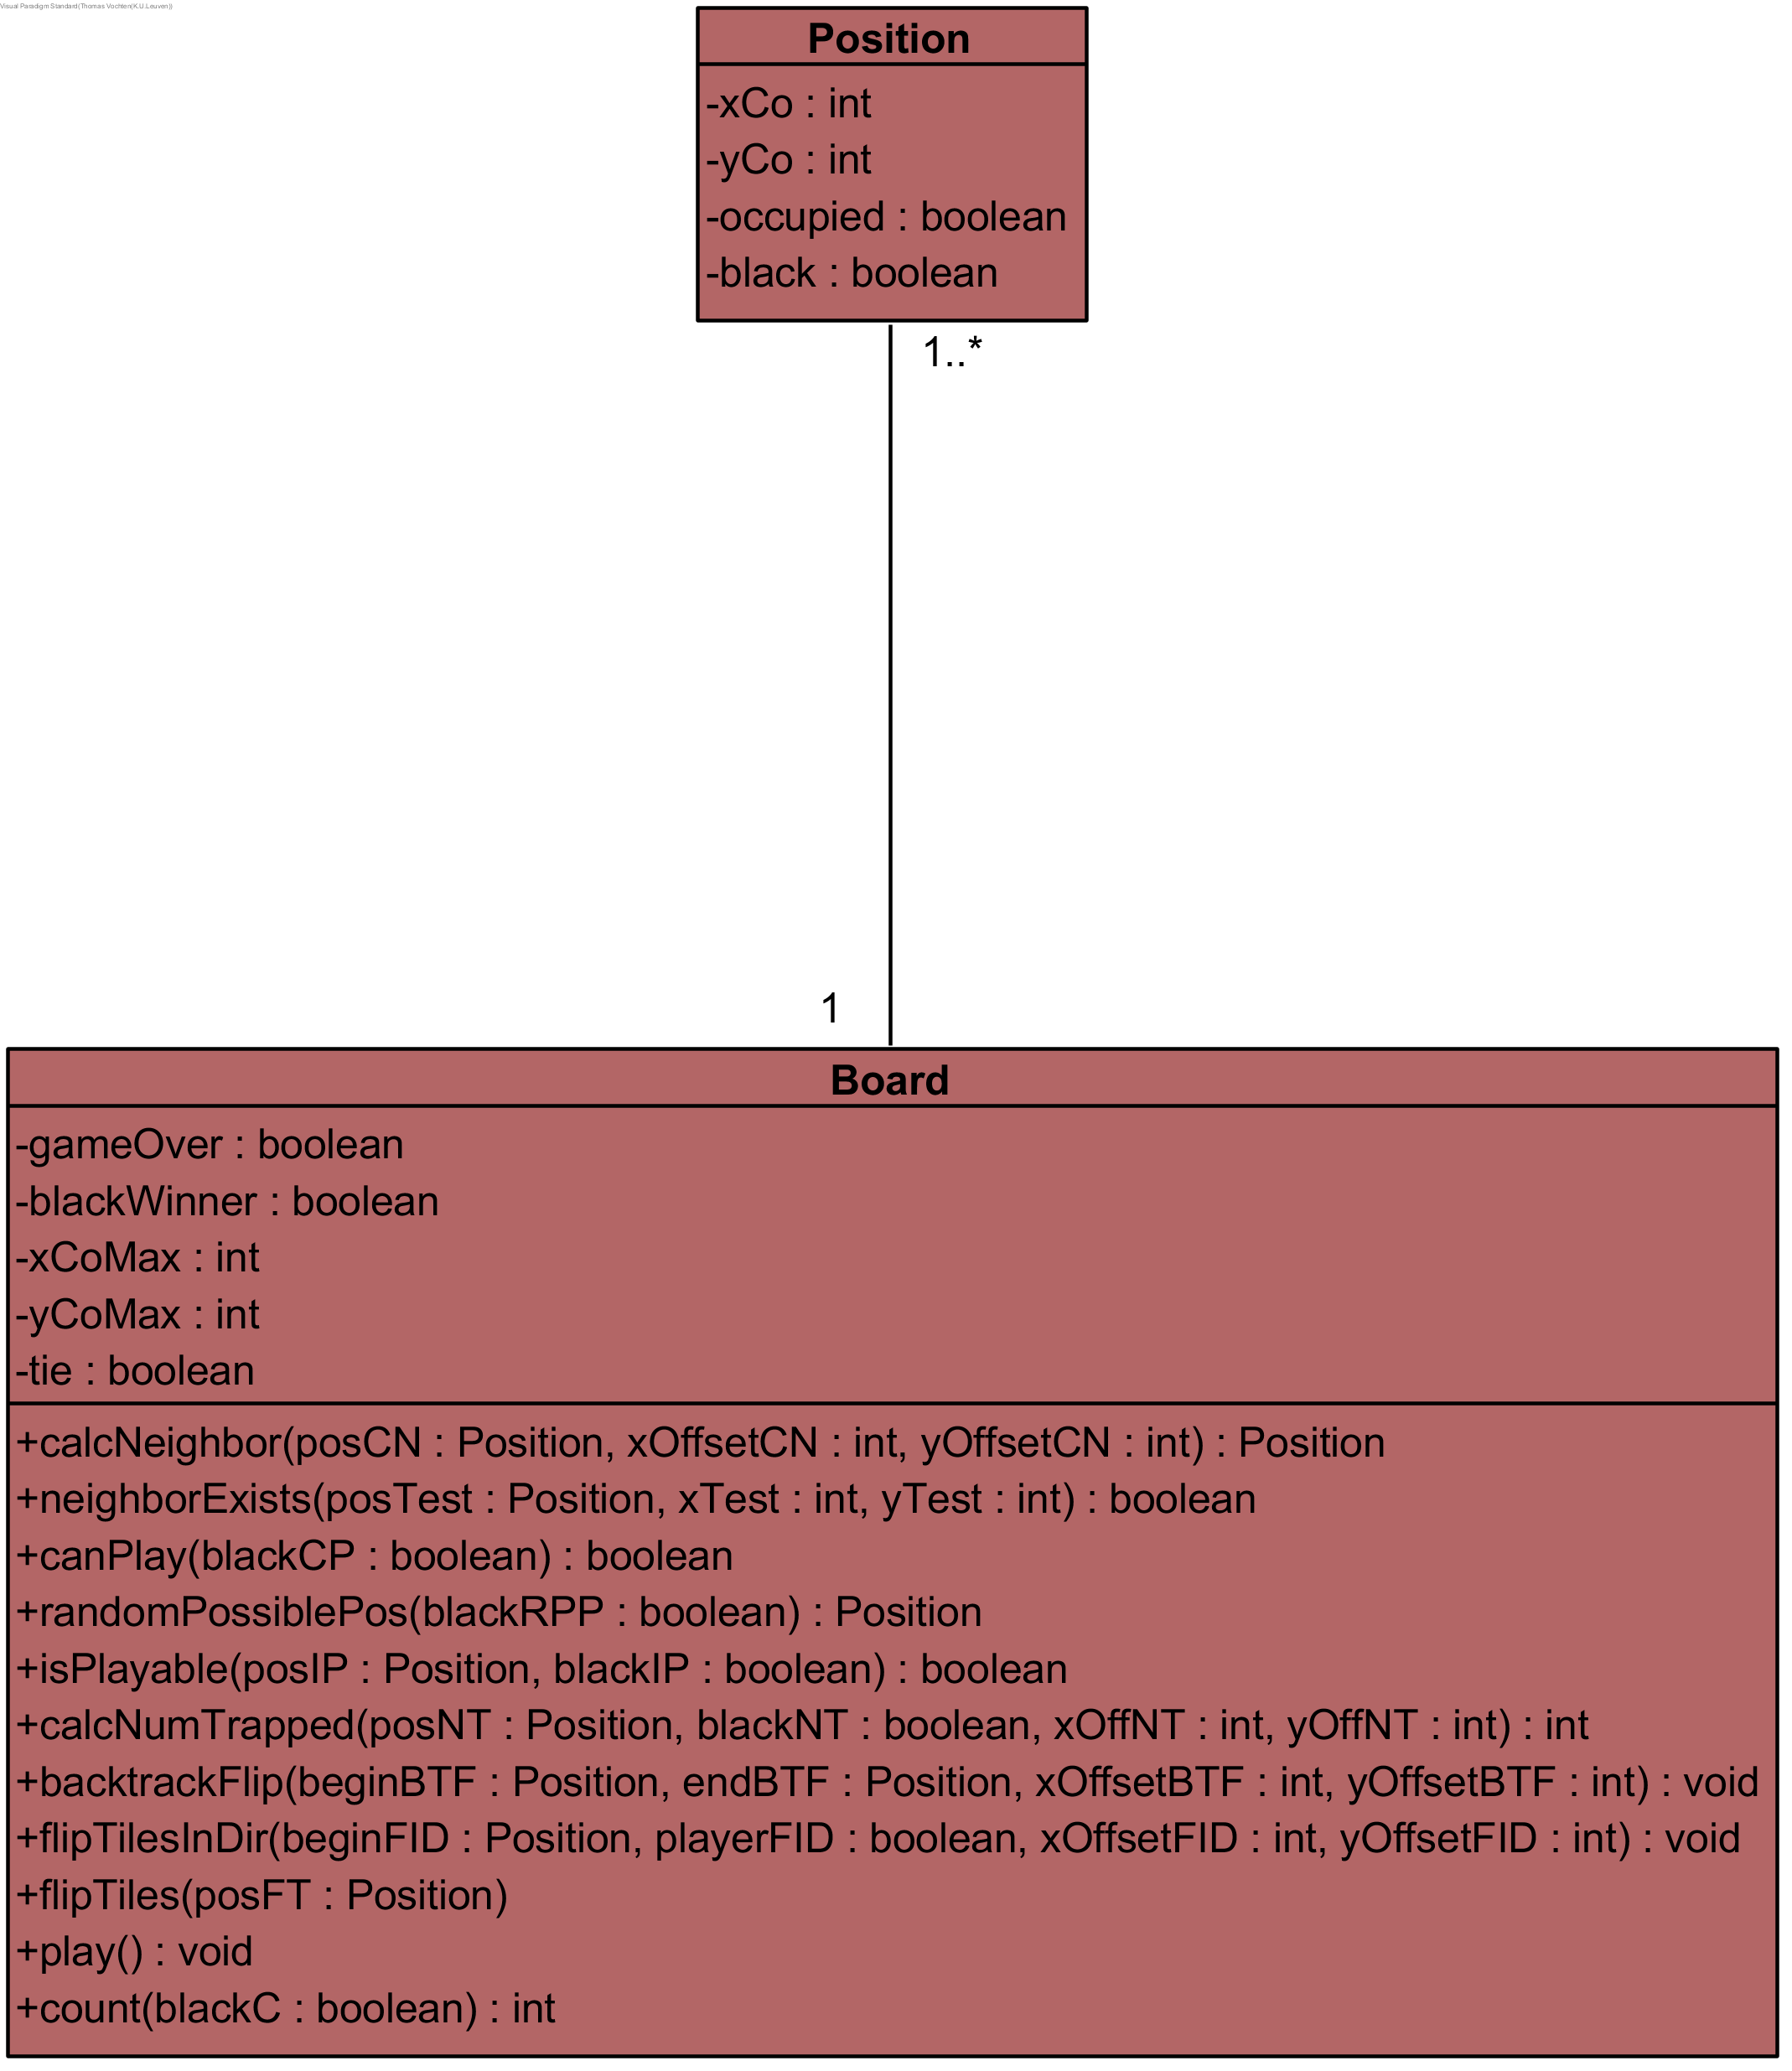
\includegraphics[width=0.77\textwidth]{chap-evaluatie/reversi-cd.png}
%	\caption{Klassediagram voor Reversi}
%	\label{fig:reversi-cd}
%\end{figure}
%
%\begin{figure}[htp]
%	\centering
%	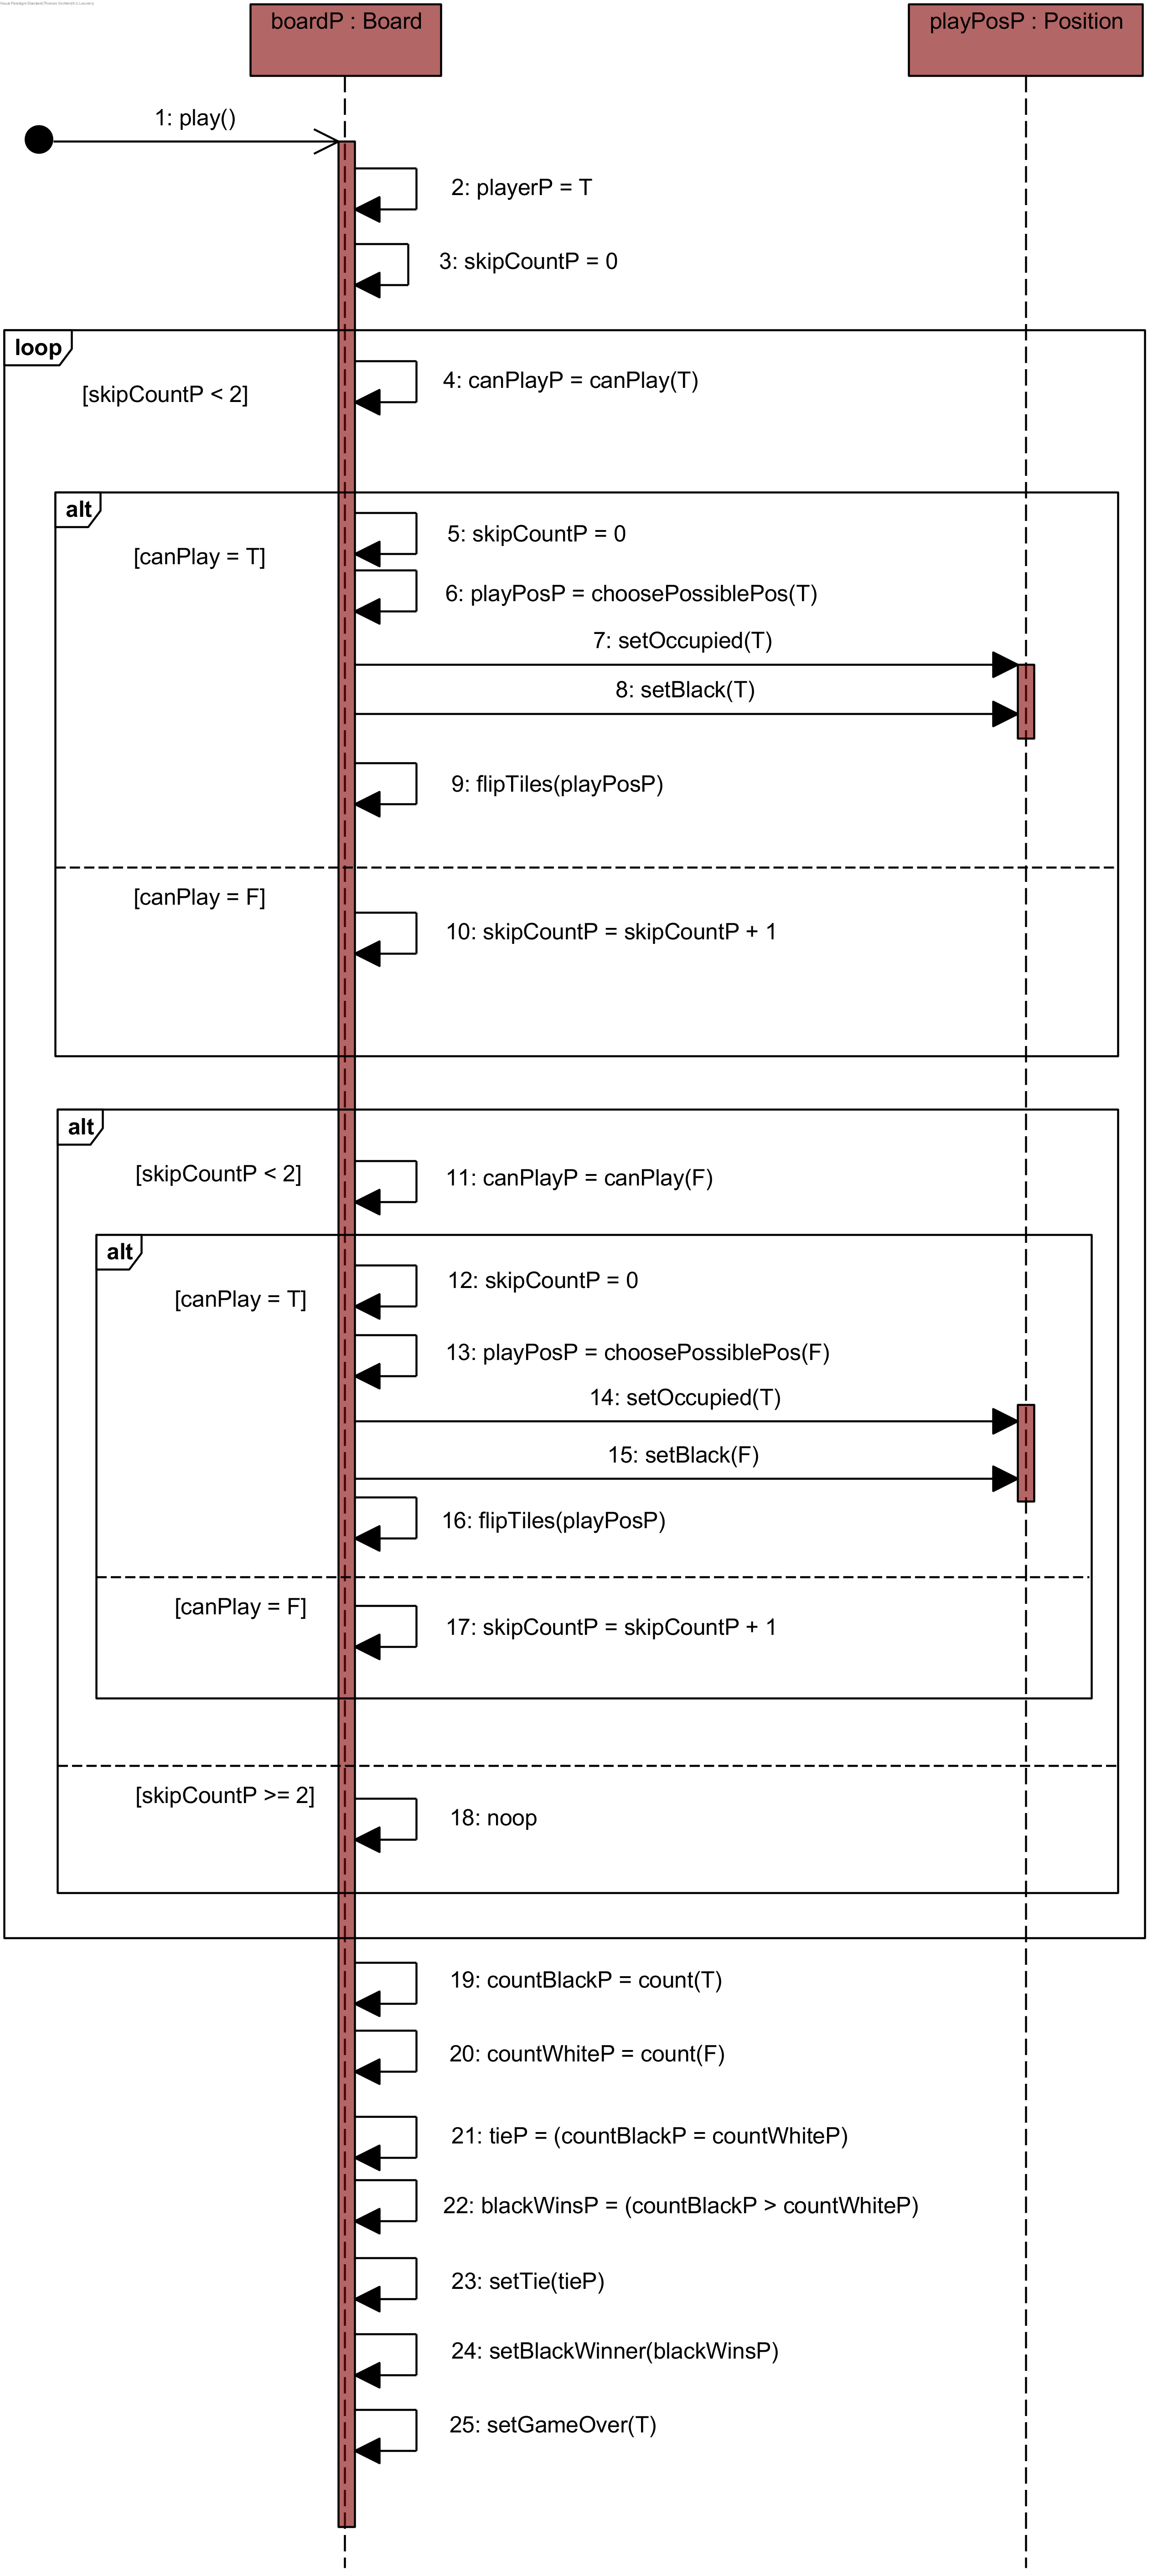
\includegraphics[width=0.825\textwidth]{chap-evaluatie/play-reversi.png}
%	\caption{Sequentiediagram voor \textit{play()}}
%	\label{fig:reversi-play}
%\end{figure}

%\begin{landscape}
%	\thispagestyle{empty}
%	\begin{figure}
%		\begin{subfigure}{\textwidth}
%			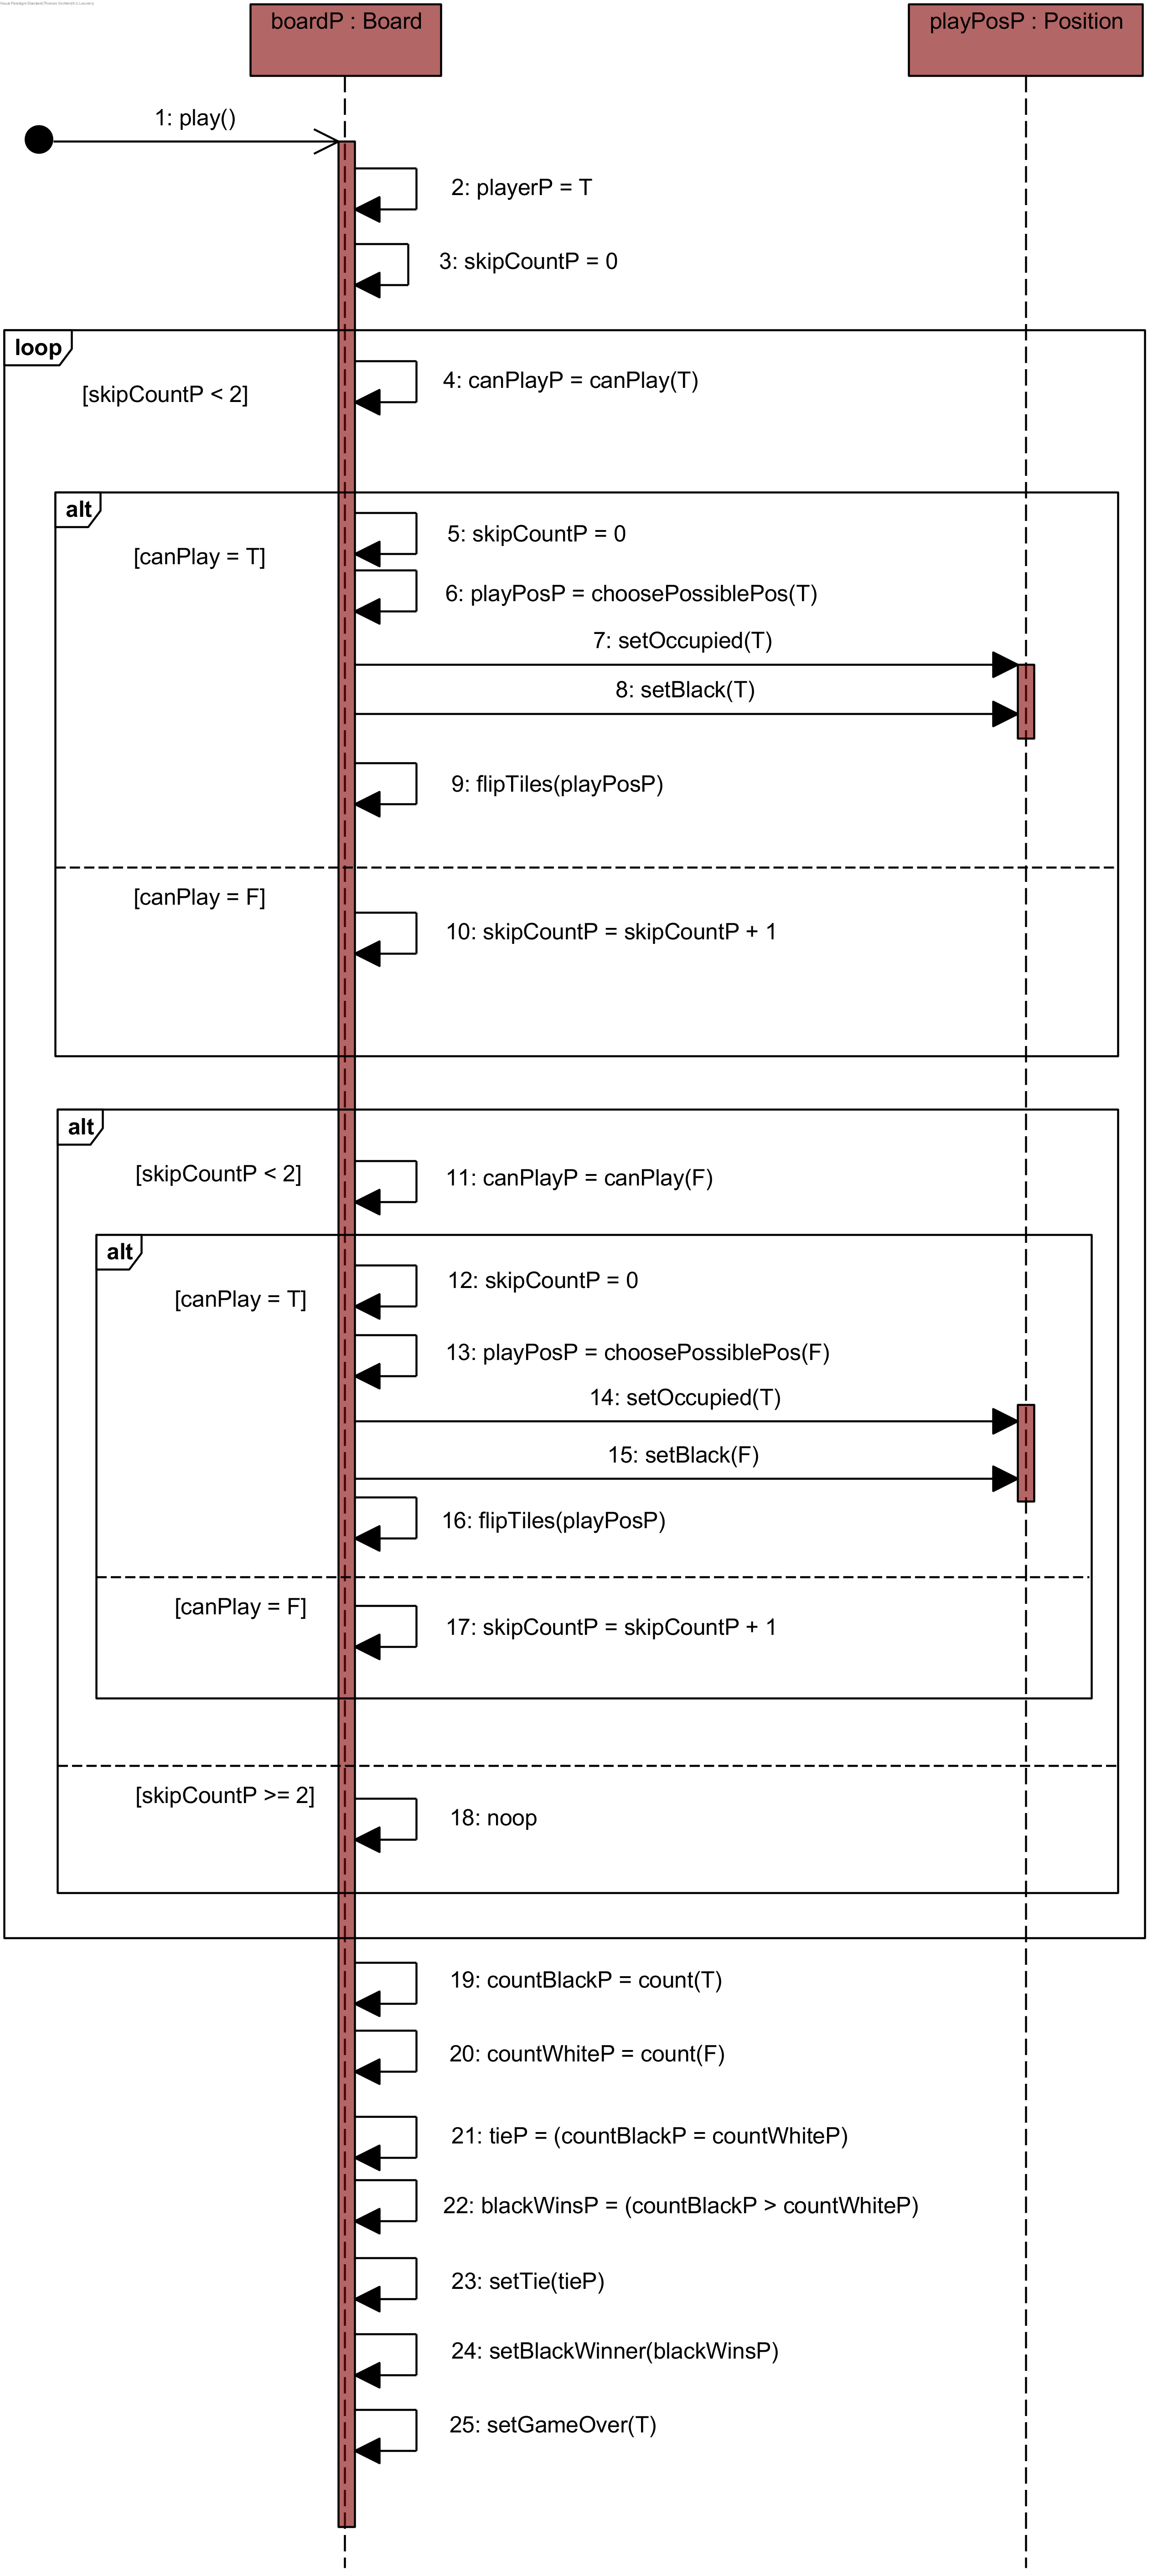
\includegraphics[width=0.6\textwidth]{chap-evaluatie/play-reversi.png}
%			\caption{Sequentiediagram voor \textit{play()}}
%			\label{fig:reversi-play}
%		\end{subfigure}
%		\begin{subfigure}{\textwidth}
%			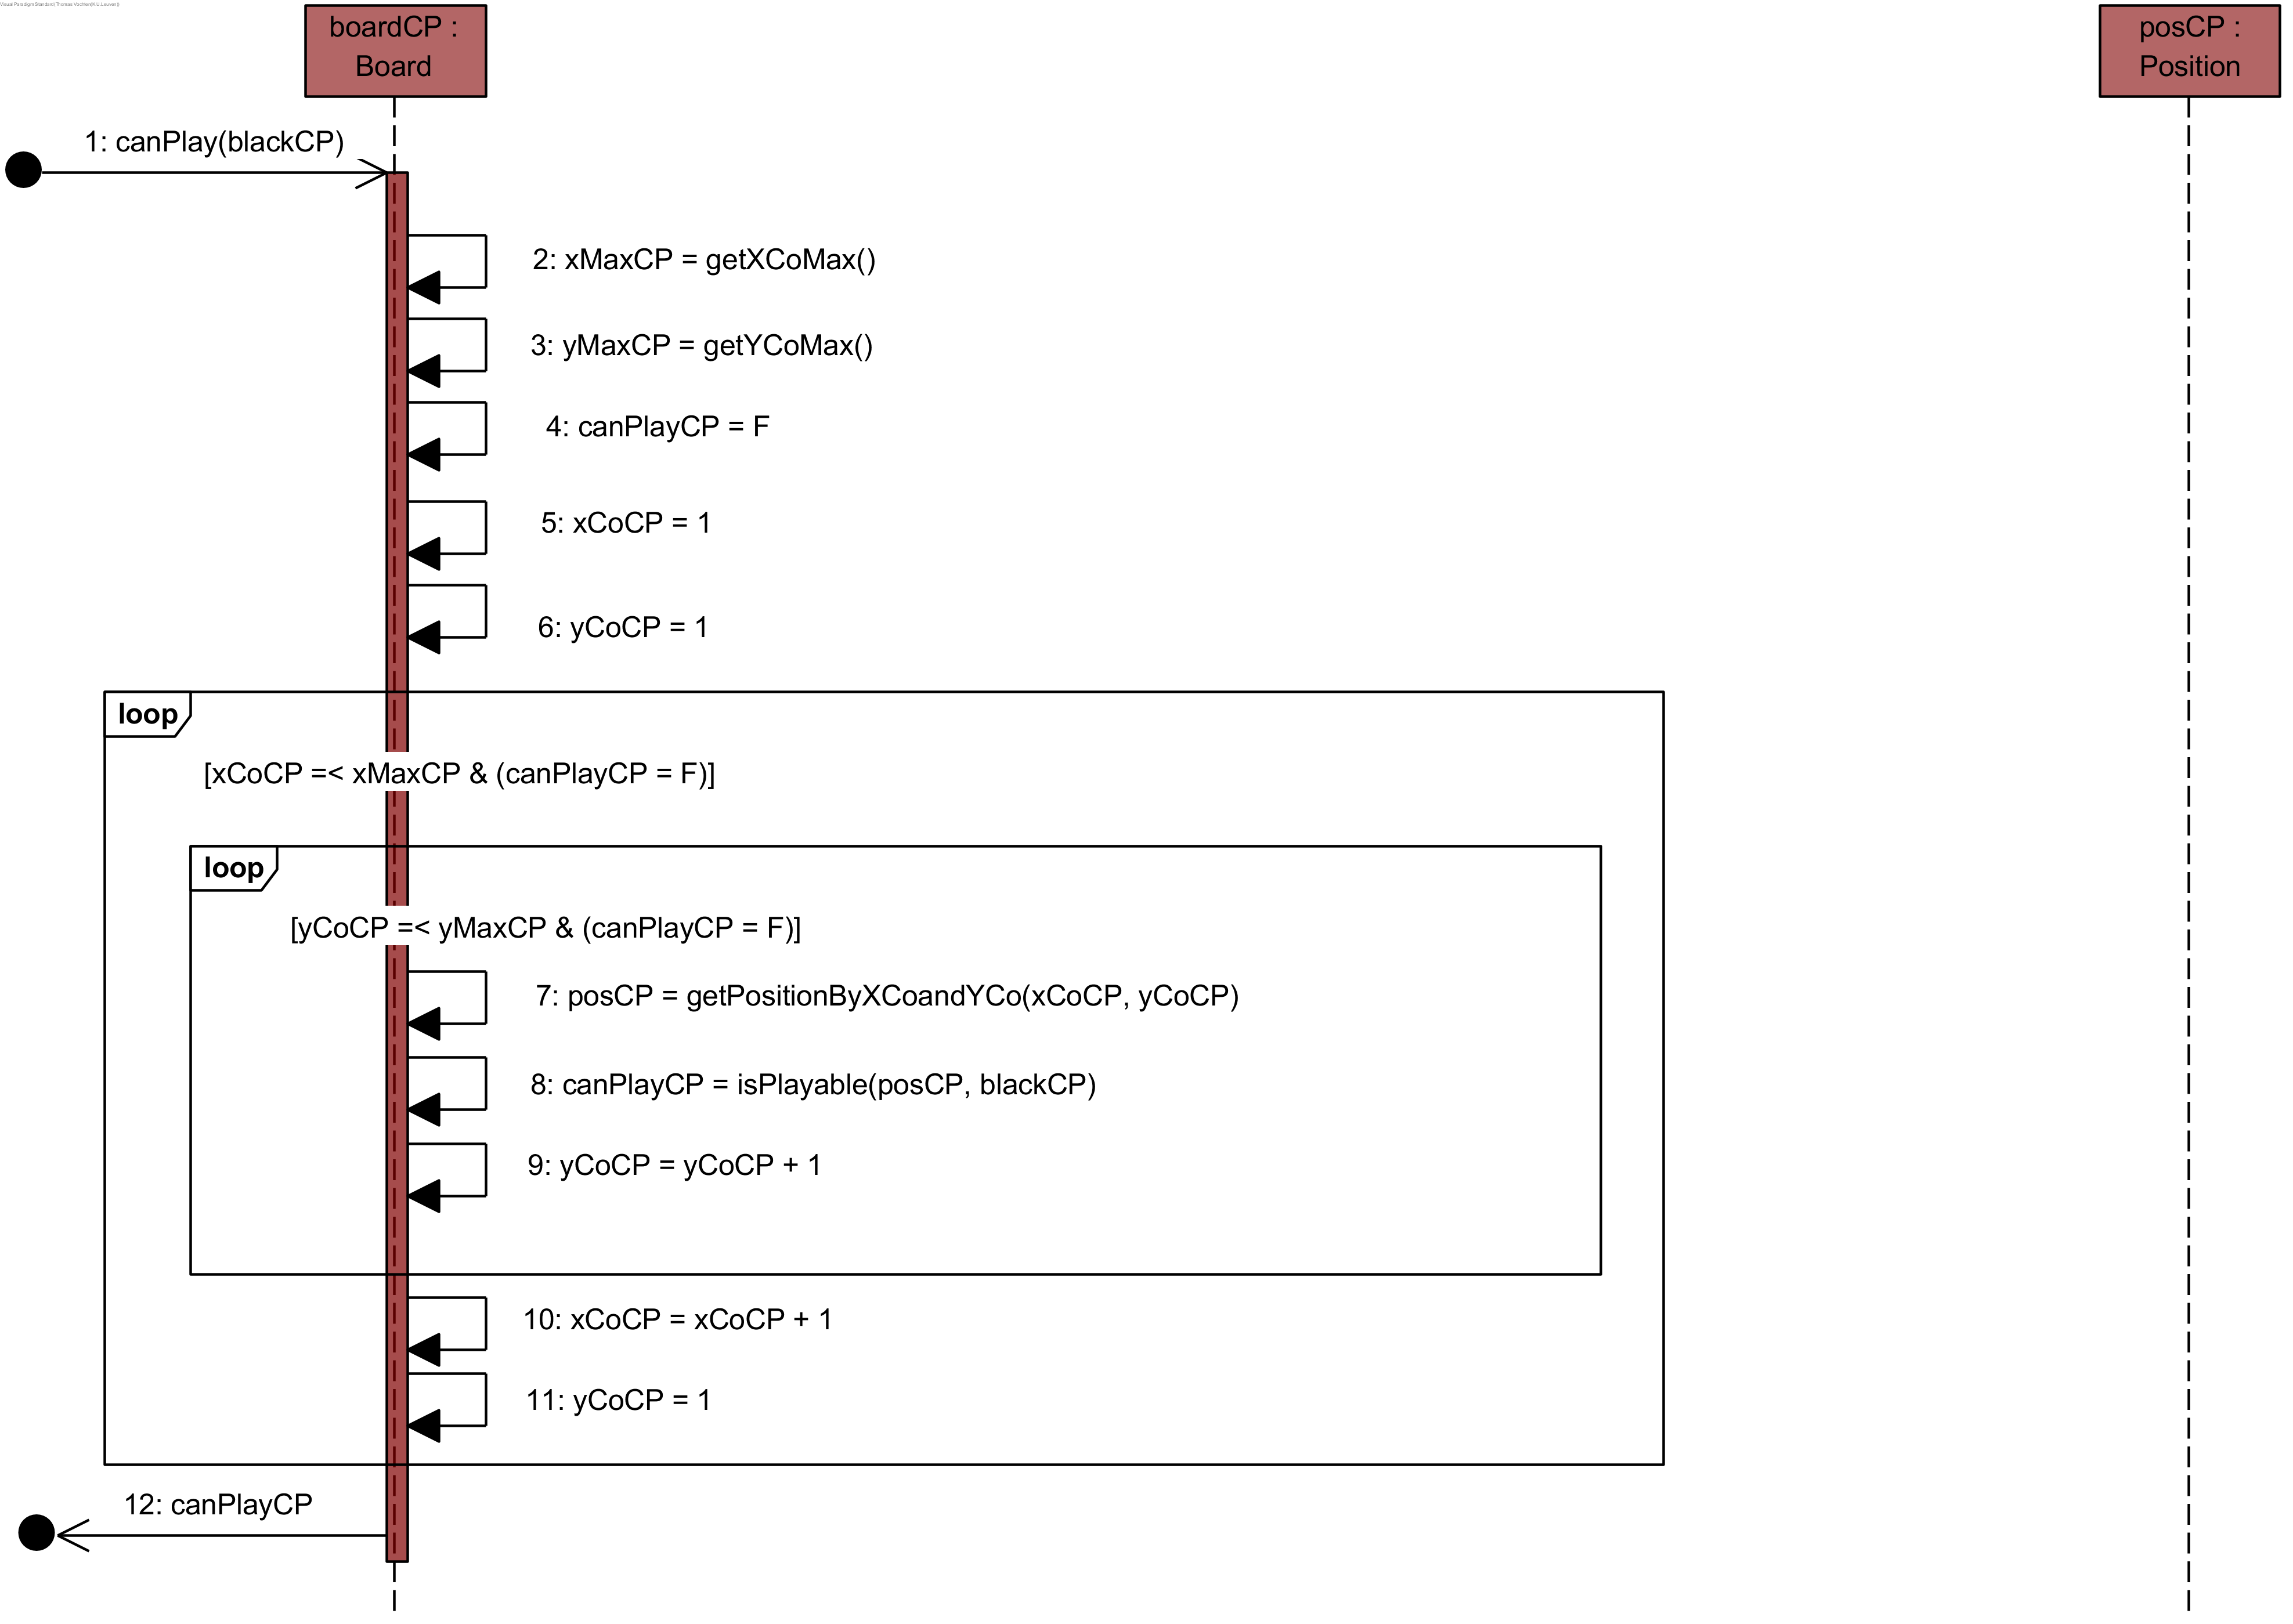
\includegraphics[width=0.9\textwidth]{chap-evaluatie/canPlay.png}
%			\caption{Sequentiediagram voor \textit{canPlay(boolean)}}
%			\label{fig:reversi-canplay}
%		\end{subfigure}
%		\caption{Sequentiediagrammen voor \textit{play()} en \textit{canPlay(boolean)}}
%		\label{fig:reversi-play-canplay}
%	\end{figure}
%\end{landscape}

\chapter{IDP-bestand voor diagram \ref{fig:new-nim} in sectie \ref{sec:new-instr}}\label{app:new-nim}

\lstinputlisting[caption=Modellering van Nim gebruikmakend van nieuwe soorten instructies]{idp-sources/new-lang.idp}\label{code:new-nim}

\chapter{IDP-bestand voor diagrammen \ref{fig:nim-assoc-cd}, \ref{fig:nim-assoc-play} en \ref{fig:nim-assoc-taketurn} in sectie \ref{sec:var-assoc}}\label{app:nim-assoc}

\lstinputlisting[caption=Modellering van Nim met variabele associaties]{chap-declaratieve-seq/nim-assoc.idp}\label{code:nim-assoc}

%\chapter{Wetenschappelijk artikel}
%
%\includepdf[pages=-]{IEEEtran/article.pdf}
%
%\chapter{Poster}
%
%\includepdf[pages=1,fitpaper]{thomas-vochten-poster.pdf}